\chapter{End-to-end Biology Network Machine Learning Project}
\label{sec:ch2}

In this chapter, we try to motivate network machine learning with some behind the scenes work, to give you a feel for what the process is really like from start to finish. While some of the material in this section might seem a little bit opaque at first, we try to keep the details lighter and the big picture in focus. You can jump around with network machine learning in a real setting, before we start jumping right into the nitty, gritty details. This will give you a chance to ensure that you have all of the dependencies set up appropriately from the beginning. Things run a lot smoother, in our experience, when you start with a working programming environment. We have the following sections:
\begin{enumerate}
    \item Section \ref{sec:ch2:bigpicture} discusses how to approach a network machine learning problem.
    \item Section \ref{sec:ch2:getdata} establishes how to set up your local environment to use this textbook, and how to grab some example data. 
    \item Section \ref{sec:ch2:prepare} details how to prepare your data for downstream analysis.
    \item Section \ref{sec:ch2:select} covers the algorithm selection process for network data.
    \item Section \ref{sec:ch2:finetune} demonstrates the tuning process for network machine learning algorithms.
    \item Section \ref{sec:ch2:discover} illustrates how we can use network machine learning to uncover new insights about network data.
\end{enumerate}

\newpage 

\section{Looking at the big picture}
\label{sec:ch2:bigpicture}


Welcome to the Neurobiology Institute! A colleague has come to you with an interesting problem. Brains consist of neurons. Different patterns in which these neurons connect produce the unique functions your brain is able to do: it is able to manage functions like breathing, as well as more active functions like moving, hearing, seeing, and higher level thought.

When they are electrically stimulated, neurons transmit that electrical signal to other neurons. This process consumes a lot of energy for your body; while the brain is only about 2\% of your weight, it consumes about 20\% of the energy your body uses per day. To keep the neurons replenished with energy (and to remove waste that the cells produce when they work), the brain has a complicated network of blood vessels. When a brain area is in use, the body dedicates blood supply to the area that will need it most.

Neurobiologists came up with a rather clever way to decipher brain activity in humans by looking at this blood flow. Using MRI, they can trace the particular areas that the blood was flowing towards. Scientists were able to demonstrate that this signal really did tend to correlate with brain activity. 

\begin{figure}[h]
    \centering
    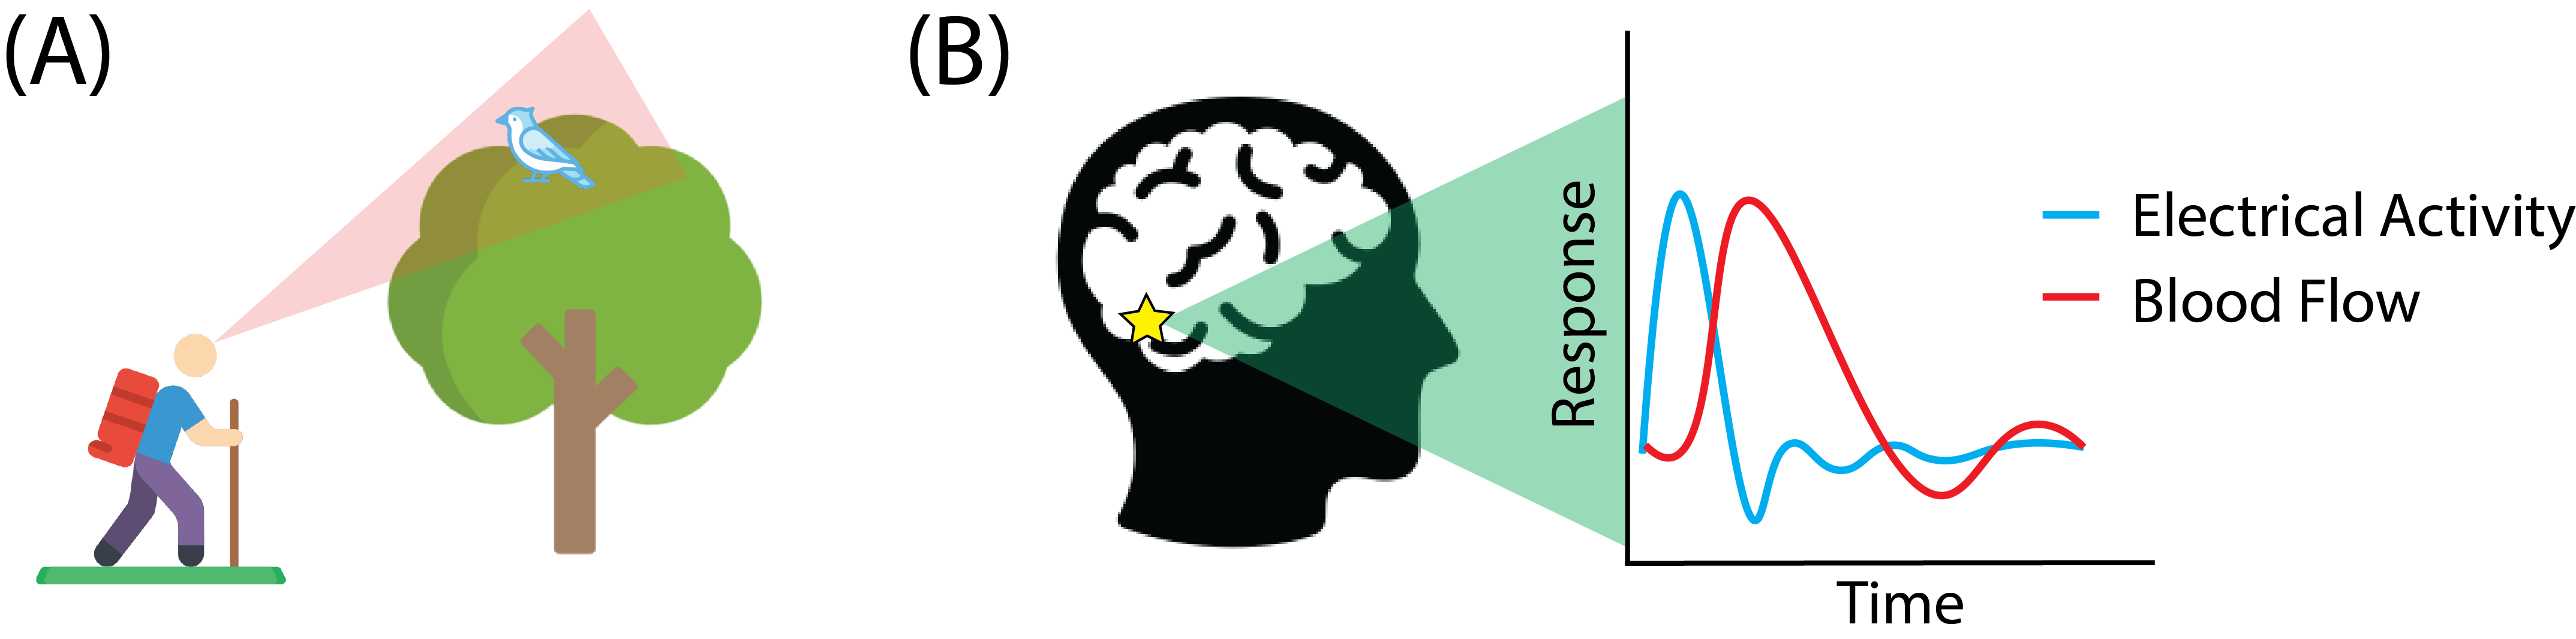
\includegraphics[width=\linewidth]{foundations/ch2/Images/fmri_bold.png}
    \caption[BOLD f-MRI]{(A) A hiker out on the trails sees a bird pirched in a tree in his field of view (faint red triangle). (B) The occipital lobe, which is responsible for sight, sits in the back of the brain (star). The presence of the bird in the field of view causes neurons to be electrically stimulated (blue line). The activity of the neurons causes the brain to send blood to the area as the neurons are stimulated (red line). While individual neurons are too small to see, the blood flow of many neurons in the brain can be picked up by the fMRI scanner.}
    \label{fig:fmri-bold}
\end{figure}

This imaging technology, known as functional MRI, has proven to be interesting to neuroscientists \cite{Poldrack2011Aug}. By measuring pairs of brain areas, researchers can see whether the two areas tend to be active together. The idea is that, perhaps, different combinations of brain areas tend to work together as a unit, allowing the complicated thought patterns that humans are capable of. By viewing the different areas of the brain as nodes of a network, and the correlations as the edges, scientists have constructed networks from this line of thinking. This area of study, called connectomics, presents an extremely network-centric area of research \cite{Munsell2018Sep}.

Your colleague has come to you with a bunch of networks from fMRI sessions, and wants to know whether there are any higher level groups of brain areas that tend to have similar activity. Can you, as a network scientist, take this network of nodes and edges, and figure out a way to break the nodes into groups of nodes which are functionally similar?

\subsection{Framing the problem}

The first question to ask your colleague is; what exactly is the objective here? In network machine learning, the choice of the model used is \emph{everything}. The model determines what sorts of questions we are capable of asking, and what sorts of \emph{answers} we are capable of learning. Asking about the objectives will directly shape which models and approaches you use.

Your colleague wants to know whether there are any sub-groups of areas that tend to behave similarly. By ``behave similarly'', what your colleague means is, are there sub-groups of brain areas that tend to work together in conjunction with other sub-groups of brain areas?

The next question is what we've tried so far. This will prevent you from repeating work, help you understand where to start approaching the problem, and give you a reference for the performance of your techniques. 

Next, you need to determine what type of network machine learning problem you have. What type of data do you have? Do you have any covariates associated with that data? What type of question do you want to answer? Do you want to test a hypothesis, or make predictions? What characteristics will your model need to reflect to be able to answer the question appropriately? Before you progress further, you should answer these questions for yourself. 

Remembering back to the types of network machine learning problems in Section \ref{sec:ch1:types}, you conclude that this is a multiple network learning problem. Your networks are non-attributed, since you only know the nodes and edges of the network. The question asks about groups of nodes and edges, and you hope to use network modelling approaches to study your problem. You are going to need to come up with a definition of what it means for pairs of areas to be similar, and you are going to want to be able to group areas in a way that is meaningful for your colleague.

\subsection{Check the assumptions}

Throughout the course of this book, we will try to keep in direct focus the assumptions being made by the techniques you might pick. You want to choose the simplest set of assumptions that can reasonably reflect the data. This means that you want to use the simplest statistical model that can answer the question you want to address. In this case, we don't care about individual brain area-to-brain area connections at all: we only care about how groups of brain areas behave in relation to other groups of brain areas. This means that we want to choose models which will allow us to learn about pairs of brain area groups, which is a very different problem from learning about individual brain areas themselves.

After talking over your understanding of the problem with your colleague, you are confident that he wants a way to be able to group brain areas together based on how similar they are, and you have the freedom to define that however you choose. You have the green light to begin coding!

\newpage
\section{Getting the data}
\label{sec:ch2:getdata}

For this section, you will start to get your hands dirty with some real network datasets. Don't be afraid to walk through these examples with your laptop in a jupyter notebook. To ease your ability to interact directly with the code of this book, we've developed a standalone \texttt{docker} container that you can use. 

\subsection{Interacting with the book via \texttt{docker}}

Getting software to run across multiple operating systems, particularly software with lots of dependencies, can range from difficult to impossible. While most of the packages required to run the contents of this book can be installed relatively easily via a combination of git, pip, and virtual environments, the easiest and fastest way to get you coding and interacting with real \texttt{python} code is \texttt{docker}. 

\texttt{docker} is a containerization utility that, in effect, allows you to run standalone software in a separate area of your computer (called a {docker container}), that allows software to operate without conflicting with your local operating system. This means that you can, with a very small number of button clicks, create deployable software that thousands of people can use at the drop of a hat. It might not be better than sliced bread, but it might be the next best thing! 

We aren't going to sit here and pretend to be the experts on docker, but fortunately the people over at docker won't leave you on your own for that one! To install docker, check out their installation guide at \cite{dockerinstall}. 

\subsubsection{Obtaining the docker container for the textbook}

Once you have docker installed on your computer, you can obtain the docker container for the book relatively easily. If you have a ubuntu/mac operating system and the docker daemon running on your computer, you can open up a terminal session and type the following command:

\begin{lstlisting}[style=bash]
$ docker pull neurodata/graph-stats-book
\end{lstlisting}

which will fetch the docker container for the book from \cite{thisbookdocker}.

This docker container contains all of the dependencies needed to run the code within this book, and will allow you to use the book in conjunction with \texttt{jupyter}. \texttt{jupyter} is a lightweight, web-based interactive computing platform that you can access through your web browser at \texttt{localhost:<port>}, where \texttt{<port>} is the port you provide to the container for execution. You can start the docker container like this:

% \begin{lstlisting}[style=bash]
% $ docker run -it --rm -p <port>:8888 neurodata/graph-stats-book \
%     jupyter-lab --ip=0.0.0.0 --port=8888 /home/book/ \
%     --NotebookApp.token="graphbook"
% \end{lstlisting}

\begin{lstlisting}[style=bash]
docker run -it -v <path/to/local/working/directory>:/home/book -p 8888:8888 neurodata/graph-stats-book \
    jupyter-lab --ip=0.0.0.0 --port=8888 /home/book/ \
    --NotebookApp.token="graphbook"
\end{lstlisting}

Which will launch a \texttt{jupyter-lab} session, and {should} automatically log you into the session in your browser. If it does not, open up a browser of your choice, and go to \texttt{localhost:<port>}, where you will be prompted to enter the log-in password for your session- that login-in password is \texttt{graphbook}, generated from \texttt{--NotebookApp.token} in the command above. If you don't know what port to choose, it's probably easiest to try \texttt{8888}, and if that doesn't work, \texttt{8889}, and keep working up until you find an open port. The port is so that your browser can communicate with the jupyter session inside the docker container (which runs jupyter internally on port \texttt{8888}), and so you are basically telling your computer that your port \texttt{<port>} should "tie in" to port \texttt{8888} in the docker container.

If you don't want to use the docker container, that's fine too: you can follow the instructions at the end in Section \ref{sec:ch2:get:install} for more details. 

\subsection{Downloading the data}

When you work with network data, it is rarely the case that the {raw data} that you will use is already a network. The \textit{raw data} is the least processed version of the data for your project, and is the information upon which the rest of your data is {derived}. A \textit{derivative} is a piece of data or information that is {derived} from the raw data. Consider, for instance, that you are investigating emailing trends for a company, and trying to see whether employees tend to email their team members more or less frequently than people outside of their team. In this case, your raw data might be a list of emails, coupled with the sender, and the recipient, of each email. You might be responsible for {preprocessing} this data to acquire a network derivative for your later analyses.

In this section, you won't worry just yet about preprocessing a raw dataset, and will instead start with some pre-prepared data. You will be working with brain networks from a human functional MRI connectome. You could navigate over to the \texttt{neurodata} website and download the file directly, but it tends to be useful to get used to how to do this programmatically. This is because if the data changes, you might want your analysis to automatically update and pertain to the latest and best version of the data at the time you execute your function. Further, if you intend your code to be reproducible, having a function which downloads and prepares the data in a way which the computer can use will simplify the process of disseminating your work. 

To begin, we'll start with a code snippet which fetches the required data for our analysis:

\begin{lstlisting}[style=python]
import os
import urllib
import boto3
from botocore import UNSIGNED
from botocore.client import Config
from graspologic.utils import import_edgelist
import numpy as np
import glob
from tqdm import tqdm

# the AWS bucket the data is stored in
BUCKET_ROOT = "open-neurodata"
parcellation = "Schaefer400"
FMRI_PREFIX = "m2g/Functional/BNU1-11-12-20-m2g-func/Connectomes/" + parcellation + "_space-MNI152NLin6_res-2x2x2.nii.gz/"
FMRI_PATH = os.path.join("datasets", "fmri")  # the output folder
DS_KEY = "abs_edgelist"  # correlation matrices for the networks to exclude

def fetch_fmri_data(bucket=BUCKET_ROOT, fmri_prefix=FMRI_PREFIX,
                    output=FMRI_PATH, name=DS_KEY):
    """
    A function to fetch fMRI connectomes from AWS S3.
    """
    # check that output directory exists
    if not os.path.isdir(FMRI_PATH):
        os.makedirs(FMRI_PATH)
    # start boto3 session anonymously
    s3 = boto3.client('s3', config=Config(signature_version=UNSIGNED))
    # obtain the filenames
    bucket_conts = s3.list_objects(Bucket=bucket, 
                    Prefix=fmri_prefix)["Contents"]
    for s3_key in tqdm(bucket_conts):
        # get the filename
        s3_object = s3_key['Key']
        # verify that we are grabbing the right file
        if name not in s3_object:
            op_fname = os.path.join(FMRI_PATH, str(s3_object.split('/')[-1]))
            if not os.path.exists(op_fname):
                s3.download_file(bucket, s3_object, op_fname)

def read_fmri_data(path=FMRI_PATH):
    """
    A function which loads the connectomes as adjacency matrices.
    """
    # import edgelists with graspologic
    # edgelists will be all of the files that end in a csv
    networks = [import_edgelist(fname) for fname in tqdm(glob.glob(os.path.join(path, "*.csv")))]
    return np.stack(networks, axis=0)
\end{lstlisting}

Now when you call \texttt{fetch\_fmri\_data()}, it creates a new directory called \texttt{datasets/fmri} in your workspace, and downloads the adjacency matrices, the standard way to represent a graph as a mathematical object, into your local directory \texttt{datasets/fmri}.

Next, we'll try to load the dataset using the \texttt{graspologic} utility, \texttt{import\_edgelist()}:

\begin{lstlisting}[style=python]
fetch_fmri_data()
As = read_fmri_data()
\end{lstlisting}

Next, let's learn some things about just one of the adjacency matrices. In network machine learning, when dealing with a new dataset, our recommendation is to {always}, {always}, start with visualization. You typically visualize network data using a heatmap. The resulting plot is shown in Figure \ref{fig:ch2:raw}(A).

\begin{lstlisting}[style=python]
from graphbook_code import heatmap

A = As[0]
ax = heatmap(A, vmin=0, vmax=1, title="Heatmap of Functional Connectome")
\end{lstlisting}

What this has done is it has plotted the adjacency matrix for the functional connectome of a human. The nodes of this network are numbered in sequential order. A heatmap is a network visualization in which the $x$ and $y$ coordinates of a given entry in the matrix indicate the pair of nodes an edge is connected to, and the color for the $(x,y)$ point in the figure indicates the weight of the edge between nodes $x$ and $y$. The edge weight is stronger if the pair of brain areas are active together more, and lower if the pair of brain areas tend to be active together less. This is real data, generated from actual fMRI scans!

One thing that we can notice from this plot is that a lot of these edges have tiny weights. Let's explore this a little bit further. 

A useful summary of the network is to look at a histogram for the edge-weights. A histogram shows the number of edges (on the vertical axis) which have a given edge weight range (indicated by the width of a particular bar on the horizontal axis). You can call this directly on the adjacency matrix (albeit flattened), and it will plot a histogram of the edge weights. We will do this using seaborn's \texttt{histplot()}:

\begin{lstlisting}[style=python]
import seaborn as sns
import matplotlib.pyplot as plt

ax = sns.histplot(A.flatten(), bins=50)
ax.set_xlabel("Edge weight")
ax.set_title("Histogram of functional connectome edge-weights")
\end{lstlisting}
A plot of the adjacency matrix's edge weights is shown in Figure \ref{fig:ch2:raw}(B). A lot of the edge-weights tend to be right around the $0.1$ to $0.5$ range, which tells us that, in general, the nodes of the network are {slightly correlated}. This means that, in general, when some node tends to be active, other nodes also tend to be active. If this were not the case, the histogram would be a bit more centered around $0.0$.

\begin{figure}[h]
    \centering
    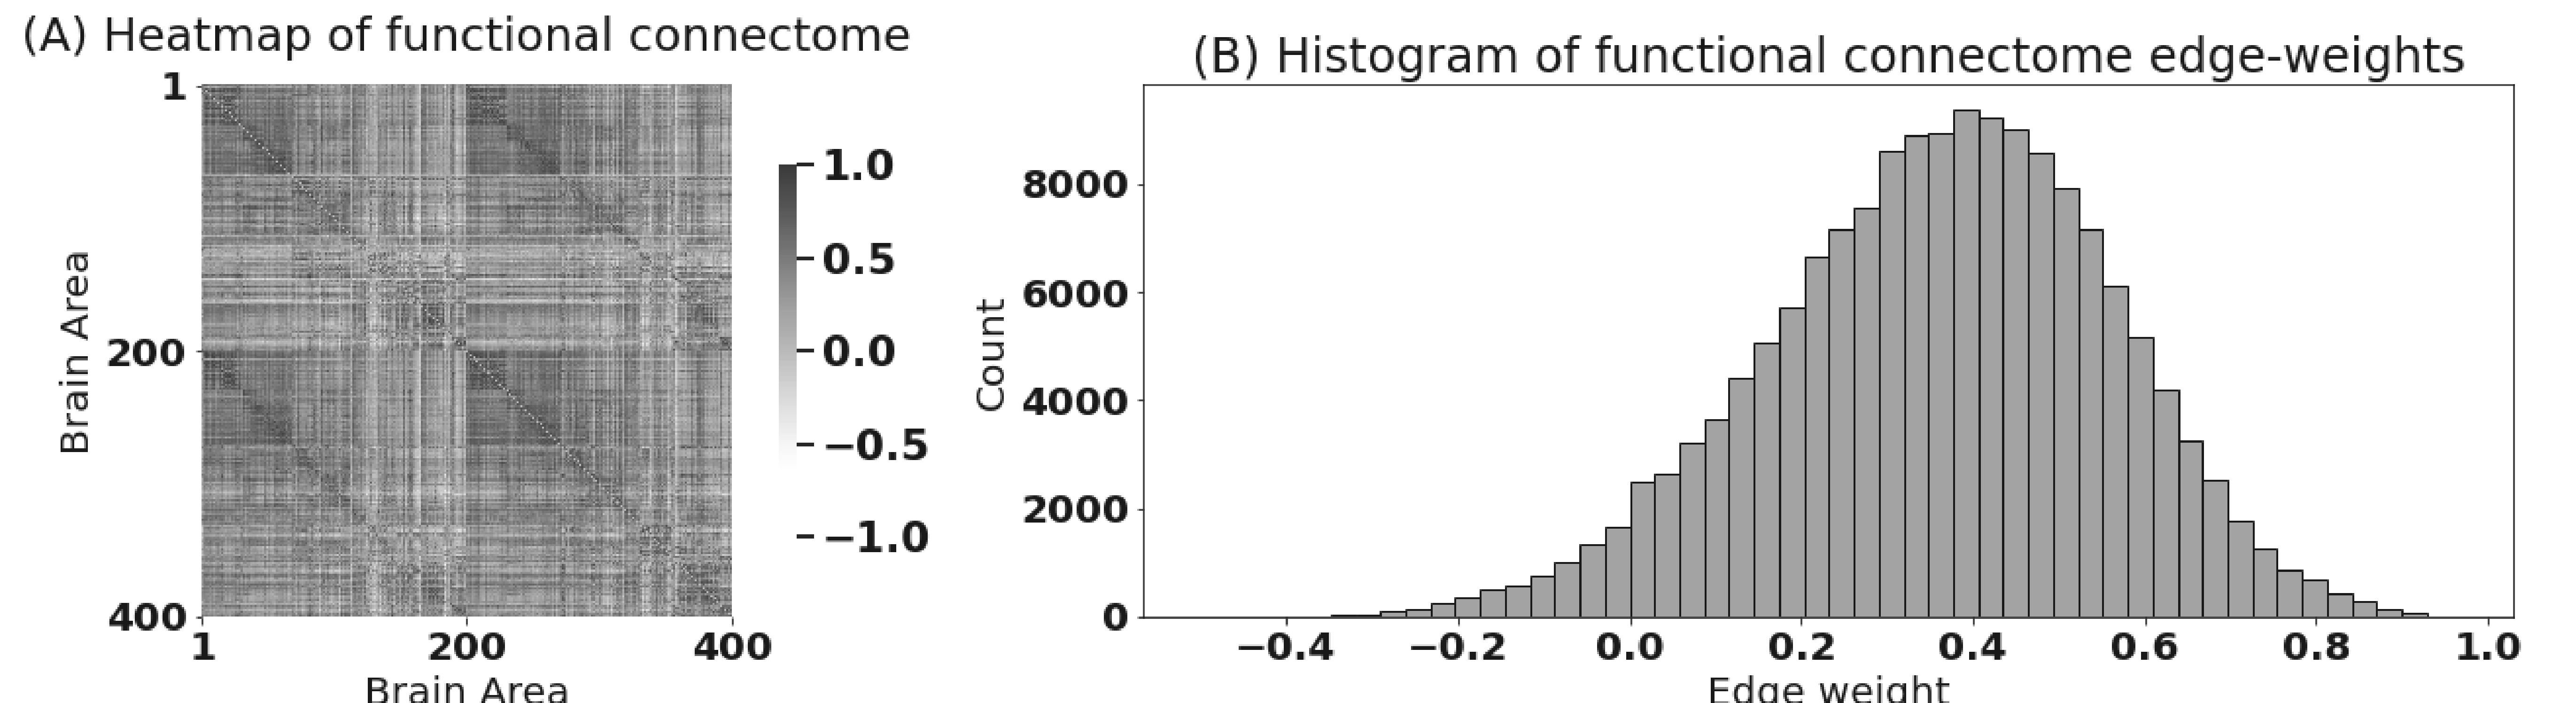
\includegraphics[width=\linewidth]{foundations/ch2/Images/raw.png}
    \caption[Visualizing connectome data]{\textbf{(A)} a raw connectome, \textbf{(B)} the raw connectome edge-weight histogram.}
    \label{fig:ch2:raw}
\end{figure}

\subsection{Create the workspace}
\label{sec:ch2:get:install}
\subsubsection{Installing the latest version of \texttt{python}}

To begin, you will need a suitable instance of \texttt{python} installed. For this book, we'll use \texttt{python 3.8}, but the most advanced version of \texttt{python3} at the time you are reading should do the trick. We will assume that you are using a Linux or UNIX-like operating system, such as OSX. If you have a Windows computer, we would recommend that you use the Docker container or the Linux subsystem module, which you can find more details about in \cite{windowsss} to interact with the codebase. Once you have this set up and up and running, you can follow the instructions below for a Debian distribution of Linux.

Once you have your computer handy, you can run the following command, which should show (ideally) \texttt{python3} has a version $\geq$\texttt{3.8.0}:

\begin{lstlisting}[style=bash]
$ python3 -V
Python 3.8.0
\end{lstlisting}

and verify that the \texttt{python} package manager, \texttt{pip}, is installed:

\begin{lstlisting}[style=bash]
$ python3 -m pip --version
pip 22.0.3 from /<user>/.virtualenvs/graph-book/lib/python3.8/site-packages/pip (python 3.8)
\end{lstlisting}

This command will print the version of \texttt{python3} and \texttt{pip} that your computer currently has installed. If it returns any version below \texttt{3.8.x} or says "command not found", you will need to obtain and install \texttt{python3} (along with the developer libraries and the package manager, \texttt{pip}) before continuing. The developer libraries are critical to ensuring that code upon which packages in \texttt{python} are based (such as the popular \texttt{numpy} numerical package) have the appropriate libraries needed to execute code written in {other} programming languages, which might be faster (for instance, \texttt{C}). 

If you have an apple computer using the OSX operating system, you can download and install an appropriate version of \texttt{python} using the \texttt{python3} guide for OSX at \cite{pythonmac} by first configuring \texttt{homebrew} and then installing python. This will also include \texttt{pip}. 

If you are using a Debian-based Linux distribution (such as Ubuntu), you can install \texttt{python3} along with the developer libraries and \texttt{pip} by typing:

\begin{lstlisting}[style=bash]
$ sudo apt-get update
$ sudo apt-get install -y python3-dev python3-pip
\end{lstlisting}

If you have a CentOS distribution (such as CentOS or Red Hat), you can install python3 along with the developer libraries and \texttt{pip} by typing:

\begin{lstlisting}[style=bash]
$ sudo yum update
$ sudo yum install -y python3-devel python3-pip
\end{lstlisting}

You should make sure that you have the most recent version of \texttt{pip} installed. To upgrade the current \texttt{pip} package, type:

\begin{lstlisting}[style=bash]
$ python3 -m pip install --user -U pip
Collecting pip
[...]
Successfully installed pip-22.0.3
\end{lstlisting}

You now have \texttt{python3}, the \texttt{python} package manager \texttt{pip}, and the \texttt{python3} developer libraries installed on your computer. 

\subsubsection{Installing fortran}

Some of the packages that you will use in the book require the system to have an appropriate version of a programming language called FORTRAN installed. FORTRAN is a numerical programming language which is very fast for mathematical computations. Fortran is included in the package \texttt{gcc}, which is a collection of compilers for many programming languages.

If you have a MAC system, you can install \texttt{gfortran} with the following command:

\begin{lstlisting}[style=bash]
$ sudo brew install gcc
\end{lstlisting}

If you have a Debian system, you can install \texttt{gfortran} with the following command:

\begin{lstlisting}[style=bash]
$ sudo apt-get update
$ sudo apt-get install gcc
\end{lstlisting}

If you have a CentOS system, you can install \texttt{gfortran} with the following command:

\begin{lstlisting}[style=bash]
$ sudo yum update
$ sudo yum install gcc
\end{lstlisting}

\subsubsection{Establishing a virtual environment}

It is often good practice in \texttt{python} to avoid installing many packages directly to \texttt{python3} itself. This is because packages in \texttt{python} do not necessarily have the same dependencies, and particular projects might require package versions that conflict with other projects you are working on. For instance, I might have a homework assignment that works only with numpy version 1.18.1, but meanwhile, a work project needs numpy version 1.22.0. For this reason, you strongly encourage you to use virtual environments.

To begin working with virtual environments in python, you will need to first obtain the \texttt{virtualenv} package:

\begin{lstlisting}[style=bash]
$ pip3 install virtualenv
Collecting package virtualenv
[...]
Successfully installed virtualenv-20.13.1
\end{lstlisting}

Once you have \texttt{virtualenv} installed, you can create your first virtual environment in python. You will first make a directory in your home directory which will allow us to keep track of your virtual environments, and then you will make a new virtual environment for the book which uses \texttt{python3}:

\begin{lstlisting}[style=bash]
$ # create a new directory for virtual environments
$ mkdir ~/.virtualenvs
$ # make a new virtual environment using python3
$ virtualenv -p python3 ~/.virtualenvs/graph-book
\end{lstlisting}

Every time you want to use run code for the book, you should first use the following command to activate the virtual environment:

\begin{lstlisting}[style=bash]
$ # activate the virtual env
$ source ~/.virtualenv/bin/activate
(graph-book) $ 
\end{lstlisting}

You should run this command before continuing to the next section.

\subsubsection{Installing the dependencies for the book}

Next, you need to install the \texttt{python} package dependencies for the book. Once you have your virtual environment activated, you will next want to grab the requirements file for the graph book, which can be obtained by typing:


\begin{lstlisting}[style=bash]
(graph-book) $ wget https://raw.githubusercontent.com/neurodata/graph-stats-book/master/requirements.txt
\end{lstlisting}

Next, you will want to install the appropriate \texttt{python} packages specified in the \texttt{requirements.txt} file, by typing:

\begin{lstlisting}[style=bash]
(graph-book) $ pip install -r requirements.txt
\end{lstlisting}

Since you are in a virtual environment, you no longer have to worry about making sure you are installing these to \texttt{python3} or \texttt{pip3}, since the virtual environment streamlines all of these function calls for us directly. Finally, you will need to install \texttt{jupyter-lab} and the ipython kernel, using the following commands:


\begin{lstlisting}[style=bash]
(graph-book) $ pip install jupyterlab ipykernel
\end{lstlisting}

We need to add your virtual environment to the ipython kernel so that jupyter lab can find it, which you can do by typing:


\begin{lstlisting}[style=bash]
(graph-book) $ python -m ipykernel install --user --name=graph-book
Installed kernelspec myenv in /home/<user>/.local/share/jupyter/kernels/graph-book
\end{lstlisting}

This will ensure that packages you install to the \texttt{graph-book} virtual environment will be findable from within jupyter.

\subsubsection{Setting up jupyter notebook}

Now that you have all your packages installed, you can finally move to starting up a notebook. Let's begin by first launching jupyter lab:

\begin{lstlisting}[style=bash]
(graph-book) $ jupyter-lab

\end{lstlisting}

Next, you want to create a new notebook using the \texttt{graph-book} module.

To verify that your notebook has the proper software installed, you will make a code cell which simply imports the \texttt{graspologic} package, by typing the following command in the top cell:

\begin{lstlisting}[style=bash]
import graspologic
graspologic.__version__
\end{lstlisting}

and then pressing the \texttt{Shift} and \texttt{Enter} keys simultaneously. Note that this cell will take a few seconds to execute successfully.


From this point forward, for each section of the book, you should be able to copy and paste code snippets section by section, and successfully reproduce the executable code contained within the book. You should take care to make sure that if you take this approach that you make sure to copy and paste all code that appears in the section, since there may be modules which are imported in above cells that are assumed to have been imported in later cells.

\newpage
\section{Preparing the data for network machine learning}
\label{sec:ch2:prepare}
Next, it's time for us to prepare our networks for machine learning algorithms. Like before, you are going to try to capture most of these with functions, because:

\begin{enumerate}
    \item Functions will make the useful data preparation code that we write usable on new networks,
    \item You will gradually build libraries of utility functions,
    \item You can use modularize these functions into other parts of your data pipeline before it gets to your algorithm, to keep a lean module-oriented design,
    \item You can easily try different transformations of the data and evaluate which ones tend to work best.
\end{enumerate}

\subsection{Data cleaning}

Most network machine learning algorithms cannot work with a node which is \emph{isolated}, meaning that the node has no edges. Let's start with fixing this. We can remove isolated nodes from the network as follows:
\begin{enumerate}
\item Compute the number of nodes each node connects to. This consists of summing the matrix along the rows (or columns). The network is undirected, which means that if a node can communicate with another node, that other node can also communicate with that node.
\item Identify any nodes which are connected to zero nodes along either the rows or columns. These are the isolated nodes.
\item Remove the isolated nodes from the adjacency matrix.
\end{enumerate}

Let's see how this works in practice. We begin by first taking the row sums of each node, which tells us how many nodes each node is connected to. Next, we remove all nodes with are not connected to any other nodes (the row and column sum are both zero) from both the adjacency matrix and the labels:

\begin{lstlisting}[style=python]
def remove_isolates(A):
    """
    A function which removes isolated nodes from the 
    adjacency matrix A.
    """
    degree = A.sum(axis=0)  # sum along the rows to obtain the node degree
    out_degree = A.sum(axis=1)
    A_purged = A[~(degree == 0),:]
    A_purged = A_purged[:,~(degree == 0)]
    print("Purging {:d} nodes...".format((degree == 0).sum()))
    return A_purged
    
A = remove_isolates(A)
# Purging 0 nodes...
\end{lstlisting}

So no isolated nodes were found, and consequently no nodes were purged. Great! What else can we do?

A common thing to do with functional MRI connectomes is to, in fact, not look at the correlations themselves, but the absolute correlations. The intuition here is that, if one node is less active when another node is active, that kind of indicates that they are still operating together. Let's take a look at how we can compute the absolute correlations:

\begin{lstlisting}[style=python]
import matplotlib.pyplot as plt
from graphbook_code import heatmap

A_abs = np.abs(A)
fig, axs = plt.subplots(1,3, figsize=(21, 6))
heatmap(A, ax=axs[0], title="Human Connectome, Raw", vmin=np.min(A), vmax=1)
heatmap(A_abs, ax=axs[1], title="Human Connectome, Absolute", vmin=np.min(A), vmax=1)
heatmap(A_abs - A, ax=axs[2], title="Difference(Absolute - Raw)", vmin=0, vmax=1)
\end{lstlisting}

Several of the values will change (the faint bands), which is indicated by larger differences from the raw to the absolute data. You can use this \texttt{heatmap} function to plot the adjacency matrix as you manipulate it later on in this section.

To streamline the process of cleaning up the raw data, you will often need to write custom data cleaners. You will want your cleaners to work seamlessly with \texttt{sklearn}'s functions, such as pipelines, and will require you to only implement three class methods: \texttt{fit()}, \texttt{transform()}, and \texttt{fit\_transform()}. By adding \texttt{TransformerMixin} as a base class, we do not even have to implement the third one! If we use \texttt{BaseEstimator} as a base class, we will also obtain \texttt{get\_params()} and \texttt{set\_params()}, which will be useful for hyperparameter tuning steps you might need in other settings. 

Here is an example cleaner class which purges the adjacency matrix of isolates and remaps the categorical labels to numbers. A key step to implementing this all as cleanly as possible is that the inputs, an adjacency matrix and a vector of node labels, are passed in as a \emph{single} tuple object. This is because \texttt{sklearn} anticipates that the return arguments from calls of \texttt{transform()} can be passed sequentially to one another.

\begin{lstlisting}[style=python]
from sklearn.base import TransformerMixin, BaseEstimator

class CleanData(BaseEstimator, TransformerMixin):

    def fit(self, X):
        return self

    def transform(self, X):
        print("Cleaning data...")
        Acleaned = remove_isolates(X)
        A_abs_cl = np.abs(Acleaned)
        self.A_ = A_abs_cl
        return self.A_

data_cleaner = CleanData()
A_clean = data_cleaner.transform(A)
# Cleaning data...
# Purging 0 nodes...
\end{lstlisting}

\subsection{Edge weight transformations}

One of the most important transformations that we will come across in network machine learning is called \emph{edge-weight transformation}. Many networks you enounter, such as the human diffusion connectome, will have edge weights which do not just take values of 1 or 0 (edge or no edge, a \emph{binary} network); rather, many networks may have discrete-weighted edges (the edges take non-negative inter values, such as 0, 1, 2, 3, ...), or decimal-weight edges (the edges take values like 0, 0.1234, 0.234, 2.4234, ...). For a number of reasons discussed in Section \ref{sec:ch4:regularization}, this is often not really a desirable characteristic.  The edges in a network might be error prone, and it might only be desirable to capture one (or a few) properties about the edge weights, rather than just leave them in their raw values. Further, a lot of the techniques we come across throughout this book might not work on networks which are not binary. For this reason, we need to get accustomed to transforming the edge weights to take new sets of values.

There are two common approaches to transform edge weights: the first is called binarization (set all of the edges to take a value of 0 or 1), and the second is called an ordinal transformation. 

\subsubsection*{Binarization of edges} 

Binarization is quite simple. It means the edges in the raw network take non-binary values (values other than just 0s and 1s), and you need them to be 0s and 1s for your algorithm. How do you solve this? 

The simplest thing to do is usually to just look at which edges take a value of zero, and keep them as zero, and then set all of the edges which take a non-zero value to one. Let's take a look at how we can implement this using \texttt{graspologic}. We first look at the network before binarization, and then after:

\begin{lstlisting}[style=python]
from graspologic.utils import binarize

threshold = 0.4
A_bin = binarize(A_clean > threshold)
\end{lstlisting}

If you plot the cleaned adjacency matrix and the binarized adjacency matrix like in Figure \ref{fig:ch2:cleaned_connectomes}, you will see that it retains a lot of the ``general idea'' of the weighted adjacency matrix, but it's a lot simpler. Whereas the edge weights in the left plot were \emph{continuous}, we've now \emph{binarized} the edges of the network to only take two possible values ($0$ or $1$). This has the effect of potentially reducing the variance (since we no longer will need as complicated of descriptions to summarize the edge-weights), but potentially increasing the bias (since we have simplified our data and have therefore potentially "thrown away" information that might be important).

Another way we could have normalized these edge weights is through something called a \emph{pass to ranks}. Through a pass to ranks, the edge weights are discarded entirely, with one exception: the edges which are non-zero are first ranked, from smallest to largest, with the largest item having a rank of one, and the smallest item having a rank of 1/(number of non-zero edges). This is called an \emph{ordinal transformation}, in that it preserves the \emph{orders} of the edge-weights, but discards all other information. The adjacency matrix of the ranked connectome is shown in Figure \ref{fig:ch2:cleaned_connectomes}(C).

\begin{lstlisting}[style=python]
from graspologic.utils import pass_to_ranks

A_ptr = pass_to_ranks(A_clean)
\end{lstlisting}
\begin{figure}[h]
    \centering
    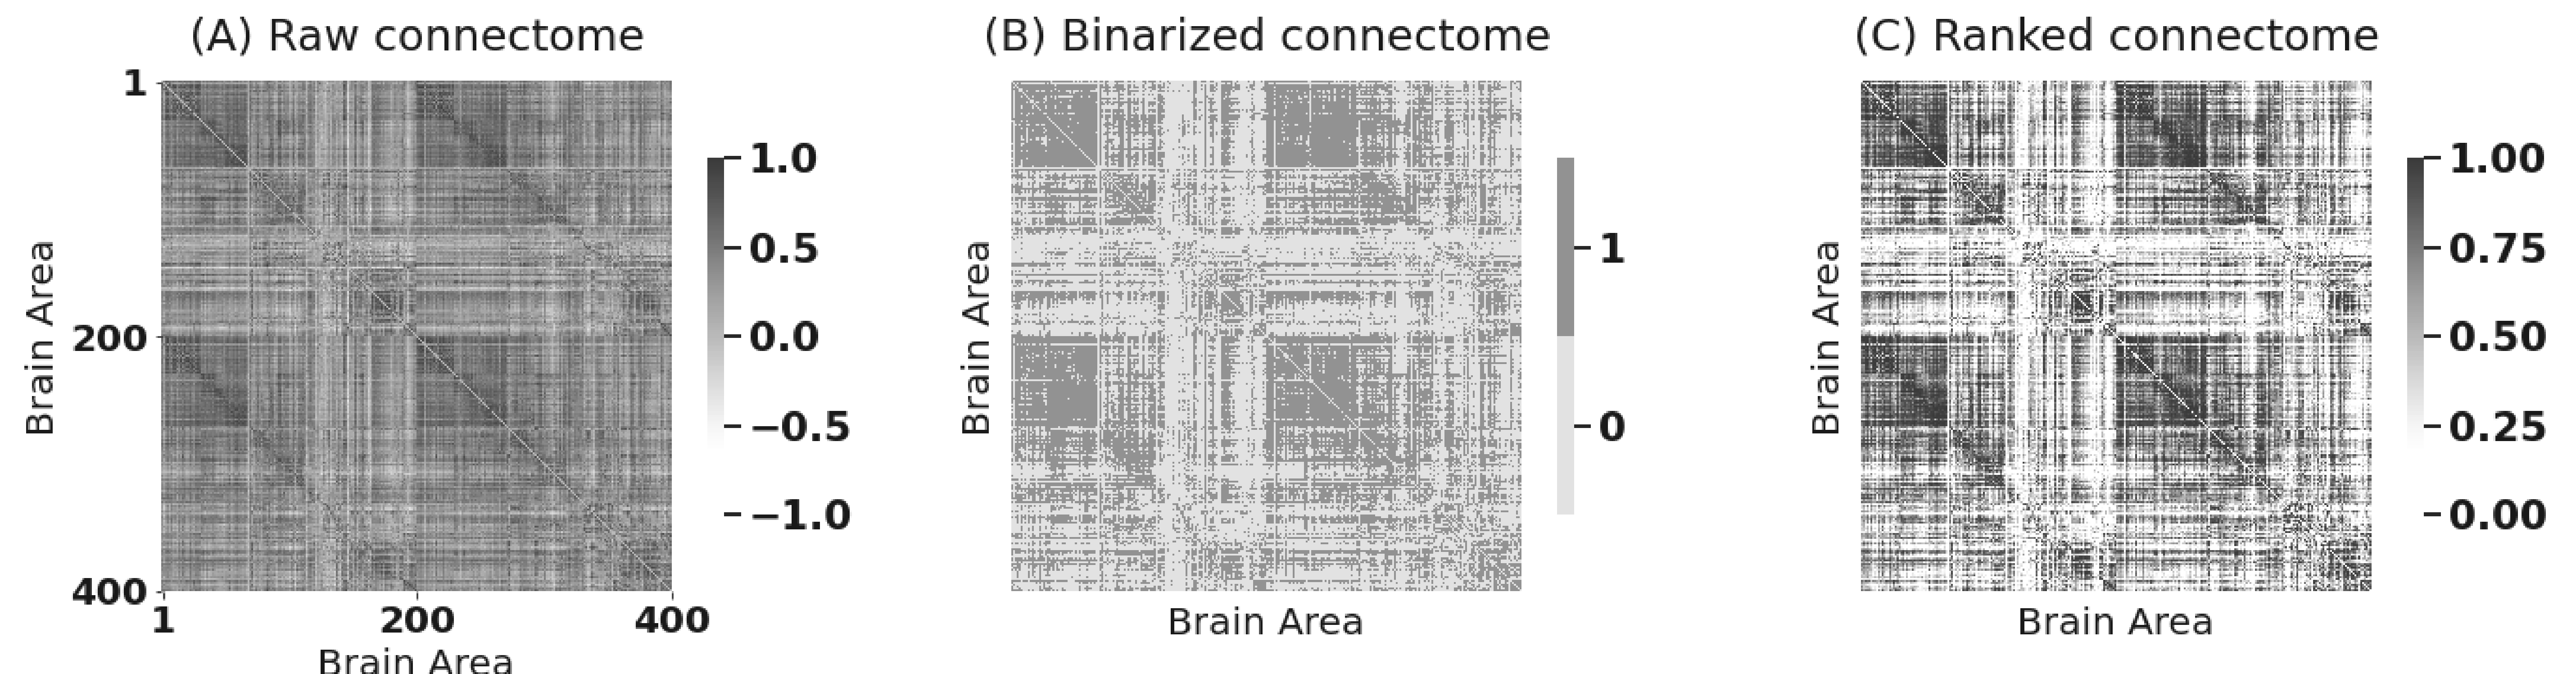
\includegraphics[width=\linewidth]{foundations/ch2/Images/cleaning_connectomes.png}
    \caption[Re-weighting connectome edge-weights]{\textbf{(A)} The cleaned connectome, before re-weighting. \textbf{(B)} The binarized connectome. \textbf{(C)} The ranked connectome.}
    \label{fig:ch2:cleaned_connectomes}
\end{figure}

This has shifted the histogram of edge-weights, as we can see by plotting a histogram:

\begin{lstlisting}[style=python]
import seaborn as sns

fig, ax = plt.subplots(2,1, figsize=(10, 10))
sns.histplot(A_clean[A_clean > 0].flatten(), ax=ax[0]);
ax[0].set_xlabel("Edge weight")
ax[0].set_title("Histogram of human connectome, non-zero edge weights");

sns.histplot(A_ptr[A_ptr > 0].flatten(), ax=ax[1]);
ax[1].set_xlabel("ptr(Edge weight)")
ax[1].set_title("Histogram of human connectome, passed-to-ranks")
\end{lstlisting}
The histograms before and after passing the adjacency matrix to ranks are shown in Figure \ref{fig:ch2:ptrhists}.

\begin{figure}[h]
    \centering
    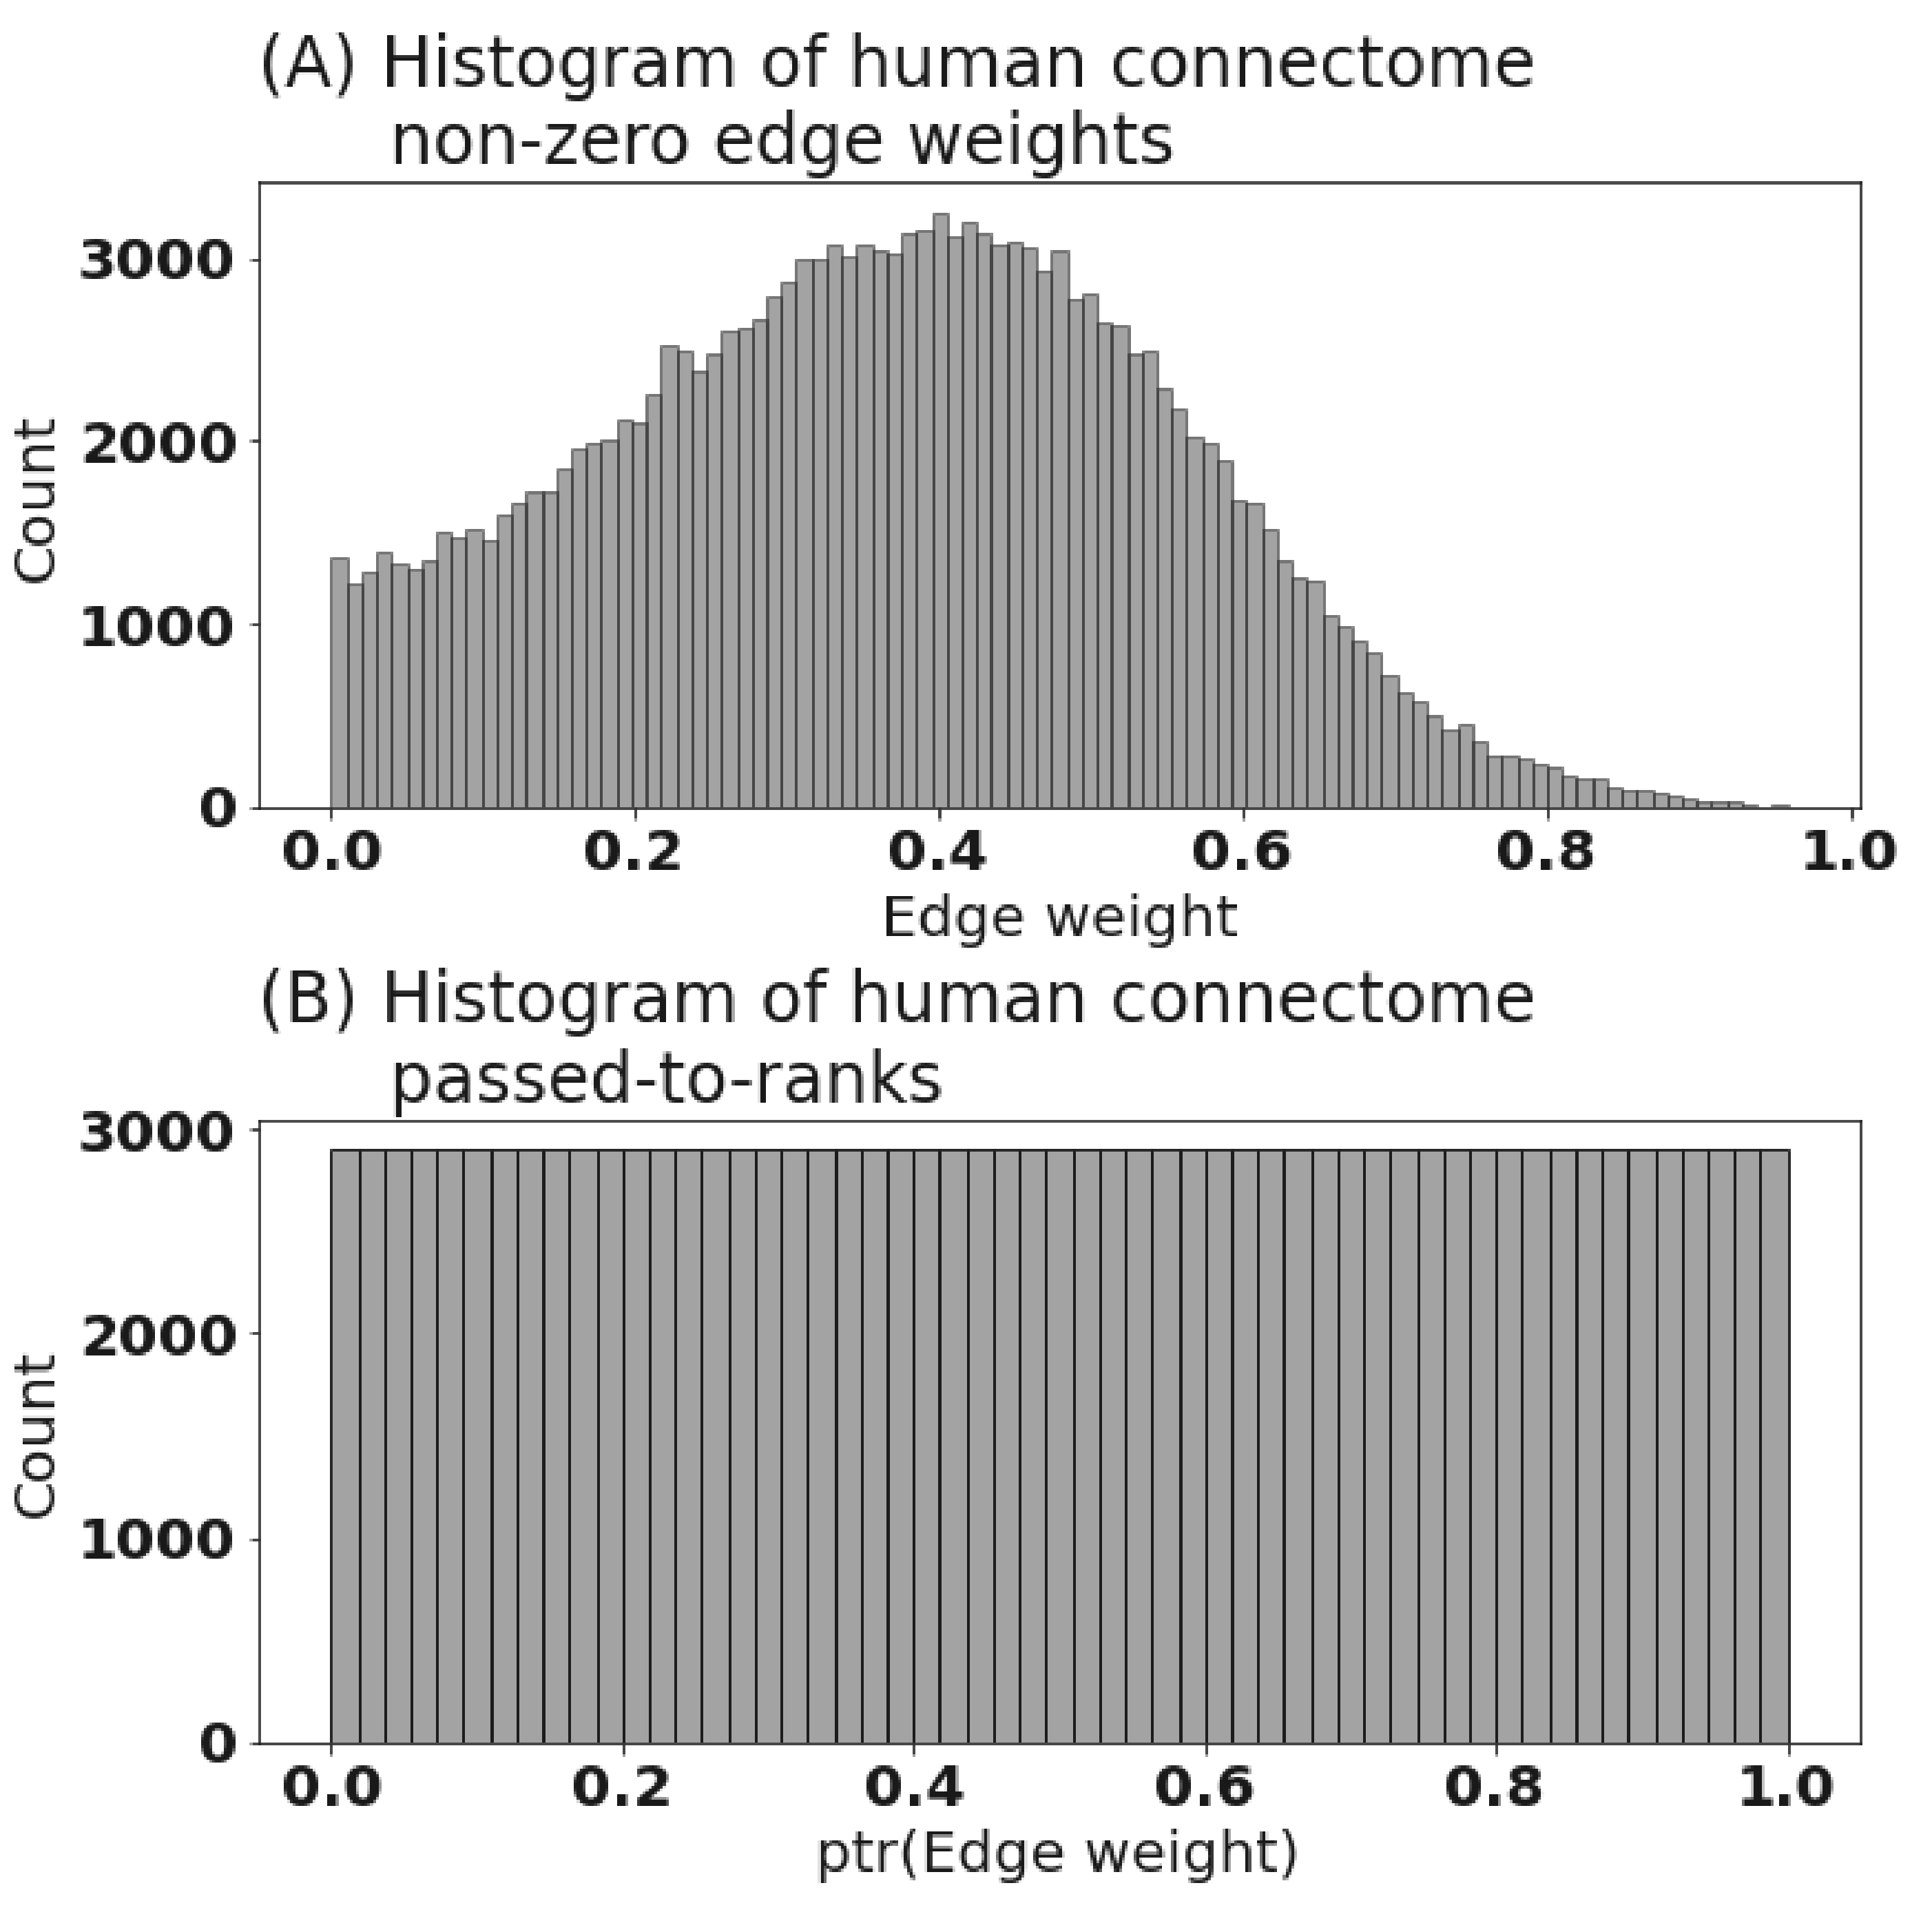
\includegraphics[width=0.6\linewidth]{foundations/ch2/Images/ptrhists.png}
    \caption[Histograms of connectome edge weights]{\textbf{(A)} Histogram of the edge-weights in the adjacency matrix before normalization. \textbf{(B)} Histogram of the edge weights in the adjacency matrix after \texttt{ptr}.}
    \label{fig:ch2:ptrhists}
\end{figure}

This has the desirable property that it bounds the network's edge weights to be between $0$ and $1$, as we can see above, which is often crucial if we seek to compare two or more networks and the edge weights are relative in magnitude (an edge's weight might mean something in relation to another edge's weight in that same network, but an edge's weight means nothing in relation to another edge's weight in a separate network). Further, passing to ranks is not very susceptible to outliers, as we will see in later chapters. 

Again, we will turn the edge-weight transformation step into its own class:

\begin{lstlisting}[style=python]
class FeatureScaler(BaseEstimator, TransformerMixin):
    
    def fit(self, X):
        return self
    
    def transform(self, X):
        print("Scaling edge-weights...")
        A_scaled = pass_to_ranks(X)
        return (A_scaled)
    
feature_scaler = FeatureScaler()
A_cleaned_scaled = feature_scaler.transform(A_clean)
# Scaling edge-weights...
\end{lstlisting}

\subsubsection*{Transformation pipelines}

As you can see, there are a number of data transformations that need to be executed to prepare network data for machine learning algorithms. One thing that might be desirable is to develop a pipeline which automates the data preparation process for you. We perform this using the \texttt{Pipeline} class from \texttt{sklearn}. The \texttt{Pipeline} class can help us apply sequences of transformations. Here is a simple pipeline for doing all of the steps we have performed so far:
\begin{lstlisting}[style=python]
from sklearn.pipeline import Pipeline

num_pipeline = Pipeline([
    ('cleaner', CleanData()),
    ('scaler', FeatureScaler()),
])

A_xfm = num_pipeline.fit_transform(A)
# Cleaning data...
# Purging 0 nodes...
# Scaling edge-weights..
\end{lstlisting}

The pipeline class takes a list of name/estimator pairs defining a sequence of steps. All but the last estimator must be transformers, which implement the \texttt{fit\_transform()} method. In our case, this is handled directly by the \texttt{TransformerMixin} base class.

When you call the \texttt{fit\_transform()} method of the numerical pipeline, it calls the \texttt{fit\_transform()} method on each of the transformers, and passes the output of each call as the parameter to the next call, until it reaches the final estimator, for which it just calls the \texttt{fit()} method. 

Next, we'll see the real handiness of the \texttt{Pipeline} module. The reason we went to lengths to define a pipeline was that we wanted to have an easily reproducible procedure that we could efficiently apply to new connectomes. This is easy to apply to the second subject in our dataset:

\begin{lstlisting}[style=python]
A_xfm2 = num_pipeline.fit_transform(As[1])
# Cleaning data...
# Purging 0 nodes...
# Scaling edge-weights...
\end{lstlisting}

\newpage
\section{Selecting and training a network machine learning model}
\label{sec:ch2:select}

So, now you've got your data loaded and pre-processed... what next?

\subsection{Generating new representations from your data}

As you were briefly introduced to in Section \ref{sec:ch1:whatis} and will cover more thoroughly in Chapter \ref{sec:ch6}, a major problem with learning from network data is that, inherently, networks in their rawest form are not tabular datasets. This means that if you want to apply any of the breadth of knowledge that has been acquired in general machine learning (which is typically designed for tabular datasets), you need to learn how to adapt your network to be compatible with tabular approaches, or learn how to adapt your general machine learning architecture for network layouts, such as adjacency matrices, which properly convey the dependences in network data. This is called \emph{representation learning}, and even neural networks typically do this under the hood with architectures like autoencoders.

As you will learn, particularly in the end of this book in Chapter \ref{sec:ch10}, the former is possible, but generally a bit more involved. The latter approach tends to be, in our opinion, a bit more straightforward at first, and is usually fantastic for most applications. So, how do you obtain a tabular representation of your dataset? 

Well, one possible thing you can do is you can use something called a spectral embedding from Chapter \ref{sec:ch6}, a technique that you will learn has a wide range of applications in network machine learning whether you are studying one network, pairs of networks, or multiple networks. Let's see what happens when we spectrally embed our connectome:

\begin{lstlisting}[style=python]
from graspologic.embed import AdjacencySpectralEmbed

embedding = AdjacencySpectralEmbed().fit_transform(A_xfm)
\end{lstlisting}

An \emph{embedding} takes the adjacency matrix, which is a matrix representation of the entire network, and turns it into a tabular array. Each row is called an \emph{estimated latent position} for a given node, and each column is called an \emph{estimated latent dimension} of the network. This means that if there are $n$ nodes, there are $n$ rows of the spectral embedding, and if there are $d$ estimated latent dimensions of the network, there are $d$ columns. Overall, the spectral embedding has taken the $n \times n$ adjacency matrix, which we \emph{can't} inherently use network machine learning algorithms on, and \emph{transformed} it into a $n \times d$ tabular array, which we \emph{can} inherently use machine learning algorithms on. We'll visualize this embedding using a \emph{pairs plot}, which as you will learn later, is a scatter plot showing where each node is a single point in the plot, and the x and y axes are different \emph{pairs} of latent dimensions for that particular node:

\begin{lstlisting}[style=python]
from graspologic.plot import pairplot

_ = pairplot(embedding, title="Spectral Embedding for connectome")
\end{lstlisting}
The results of this pairs plot are shown in Figure \ref{fig:ch2:pairplots}(A).

As it turns out, this particular representation of the adjacency matrix through the \emph{spectral embedding} can, optionally, be tied into a statistical model if you make some assumptions; particularly, those of the stochastic block model described in Section \ref{sec:ch5:sbm}. Basically, the stochastic block model says that each node is a member of a subgroup, called a \emph{community}, and its connectivity to other nodes in the network is dictated by which community it is a member of, and which community the other node is a member of. This sounds a \emph{lot} like the question that your colleague wanted you to approach, since he wanted a way to take the nodes of the network and form ``functionally similar'' subgroups from them. 

\subsection{Using your representations to learn new features from the network}

Now that we have a tabular representation of the data, we can take attempt to use the intuition and assumptions of the stochastic block model to cluster our nodes. Let's see what happens when we apply \texttt{KMeans} to our data:
\begin{lstlisting}[style=python]
from sklearn.cluster import KMeans

labels = KMeans(n_clusters=2).fit_predict(embedding)
_ = pairplot(embedding, labels=labels, legend_name="Predicter Clusters", 
                 title="KMeans clustering")
\end{lstlisting}

The results of this pairs plot are shown in Figure \ref{fig:ch2:pairplots}(B).
\begin{figure}
    \centering
    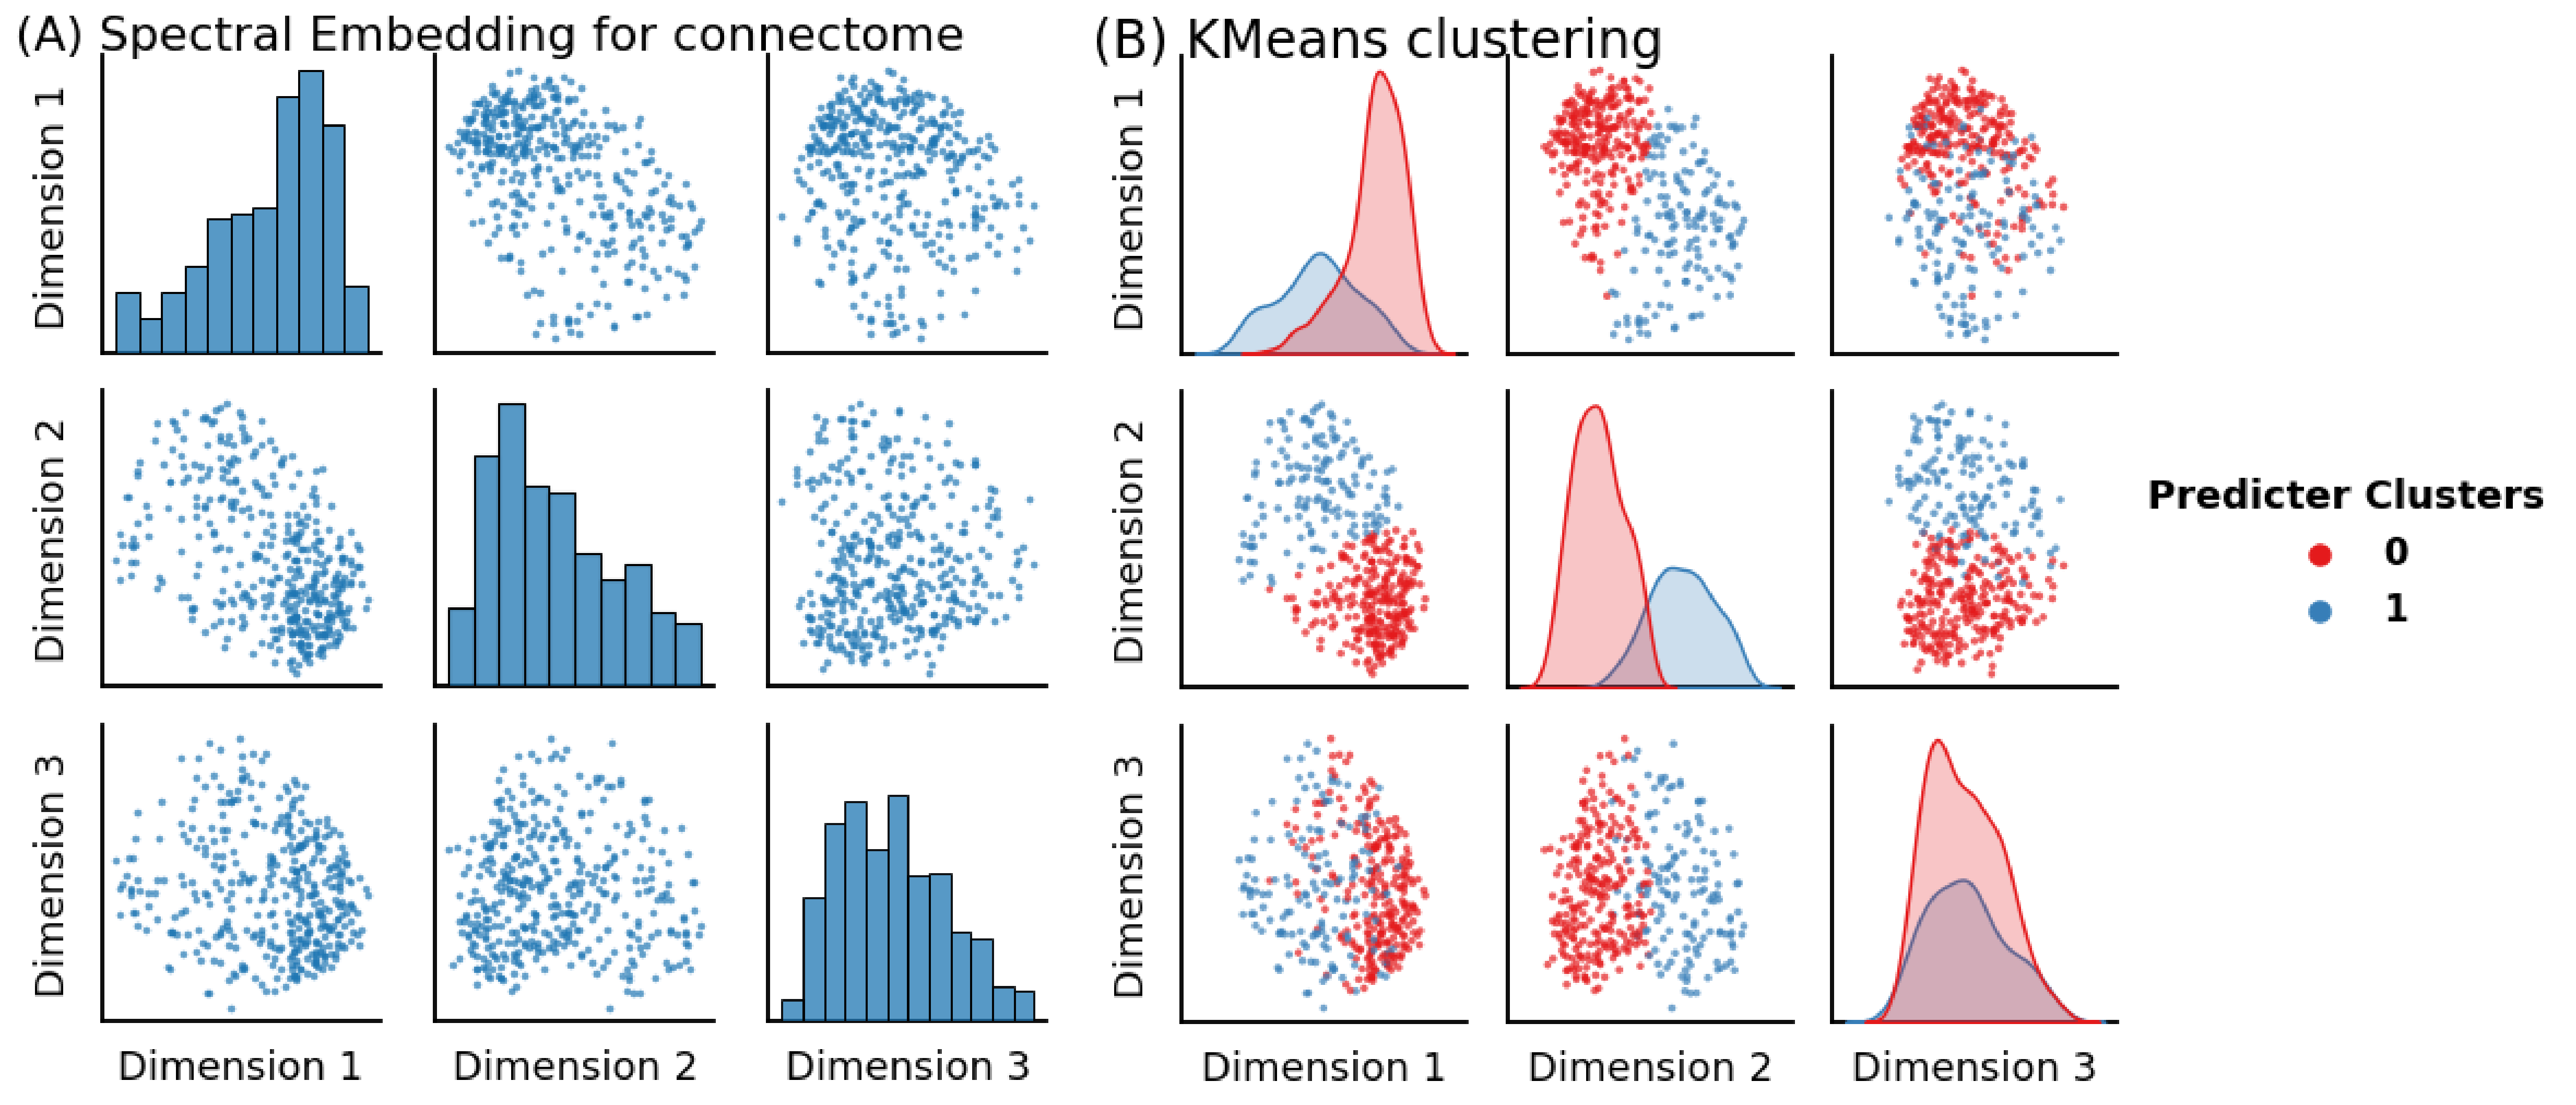
\includegraphics[width=\linewidth]{foundations/ch2/Images/pairplots.png}
    \caption[The pairs plot for embedded connectomes]{\textbf{(A)} shows the  pairs plot for the estimated latent dimensions. \textbf{(B)} shows the  pairs plot with predicted communities of nodes via \texttt{KMeans} with $2$ clusters.}
    \label{fig:ch2:pairplots}
\end{figure}
So, it looks like the $k$-means was able to learn $2$ clusters from our dataset. These clusters are indicated by the ``blobs'' of points that are red or blue, respectively.

If you're careful, you'll notice we did something a little weird here. Why did we choose $2$? Why not $5$? Why not $8$? We chose $2$ here somewhat arbitrarily. In general, when you don't know what to expect from your data (we didn't know what to expect here, other than that we wanted a modestly sized way to group the nodes up), it's a good idea to use quantitative means to make these determinations for you. 

With \texttt{KMeans}, we can use something called the silhouette score to do this for us. You choose the optimal number of clusters as the clustering with the highest silhouette score. You'll learn a lot more about the silhouette score when you learn about community detection in Section \ref{sec:ch7:comm_detect}. \texttt{graspologic} makes this process pretty straightforward with a \texttt{KMeansCluster} class, which uses the silhouette score under the hood:

\begin{lstlisting}[style=python]
from graspologic.cluster import KMeansCluster

labels = KMeansCluster(max_clusters=10).fit_predict(embedding)
_ = pairplot(embedding, labels=labels, title="KMeans clustering, automatic selection", 
                 legend_name="Predicted Clusters")
\end{lstlisting}
Unlike the previous approach, it looks like with silhouette score selection, we ended up with $5$ clusters being optimal, not $2$. The pairs plot for the embedded data with the new labels are in Figure \ref{fig:ch2:pairplots_impute}(A). Note that you might get a different number of estimated clusters than we did, because there is some randomness in the unsupervised learning procedure that we used here.

So, what about other possible approaches? Unless you are pretty confident that the clusters you are looking for have ``blobs'' that are totally spherically symmetric (basically, they look like ``balls'' in the dataset), $k$-means can be a pretty bad idea. As you'll learn later, another strategy called the gaussian mixture model, or \texttt{GMM}, handles this a bit more elegantly, and allows your cluster blobs to be pretty much any ellipse-like shape. We can use \texttt{GMM} and automatically select the number of clusters using the Bayesian Information Criterion, or BIC, with \texttt{AutoGMMCluster}:
\begin{lstlisting}[style=python]
from graspologic.cluster import AutoGMMCluster

labels = AutoGMMCluster(max_components=10).fit_predict(embedding)
_ = pairplot(embedding, labels=labels, title="AutoGMM Clustering", 
                  legend_name="Predicted Clusters")
\end{lstlisting}
The pairs plot for the embedded data with the labels determined by \texttt{GMM} in Figure \ref{fig:ch2:pairplots_impute}(B). It looks like GMM actually found $4$ clusters to be a bit more optimal than $3$ clusters. 

\begin{figure}
    \centering
    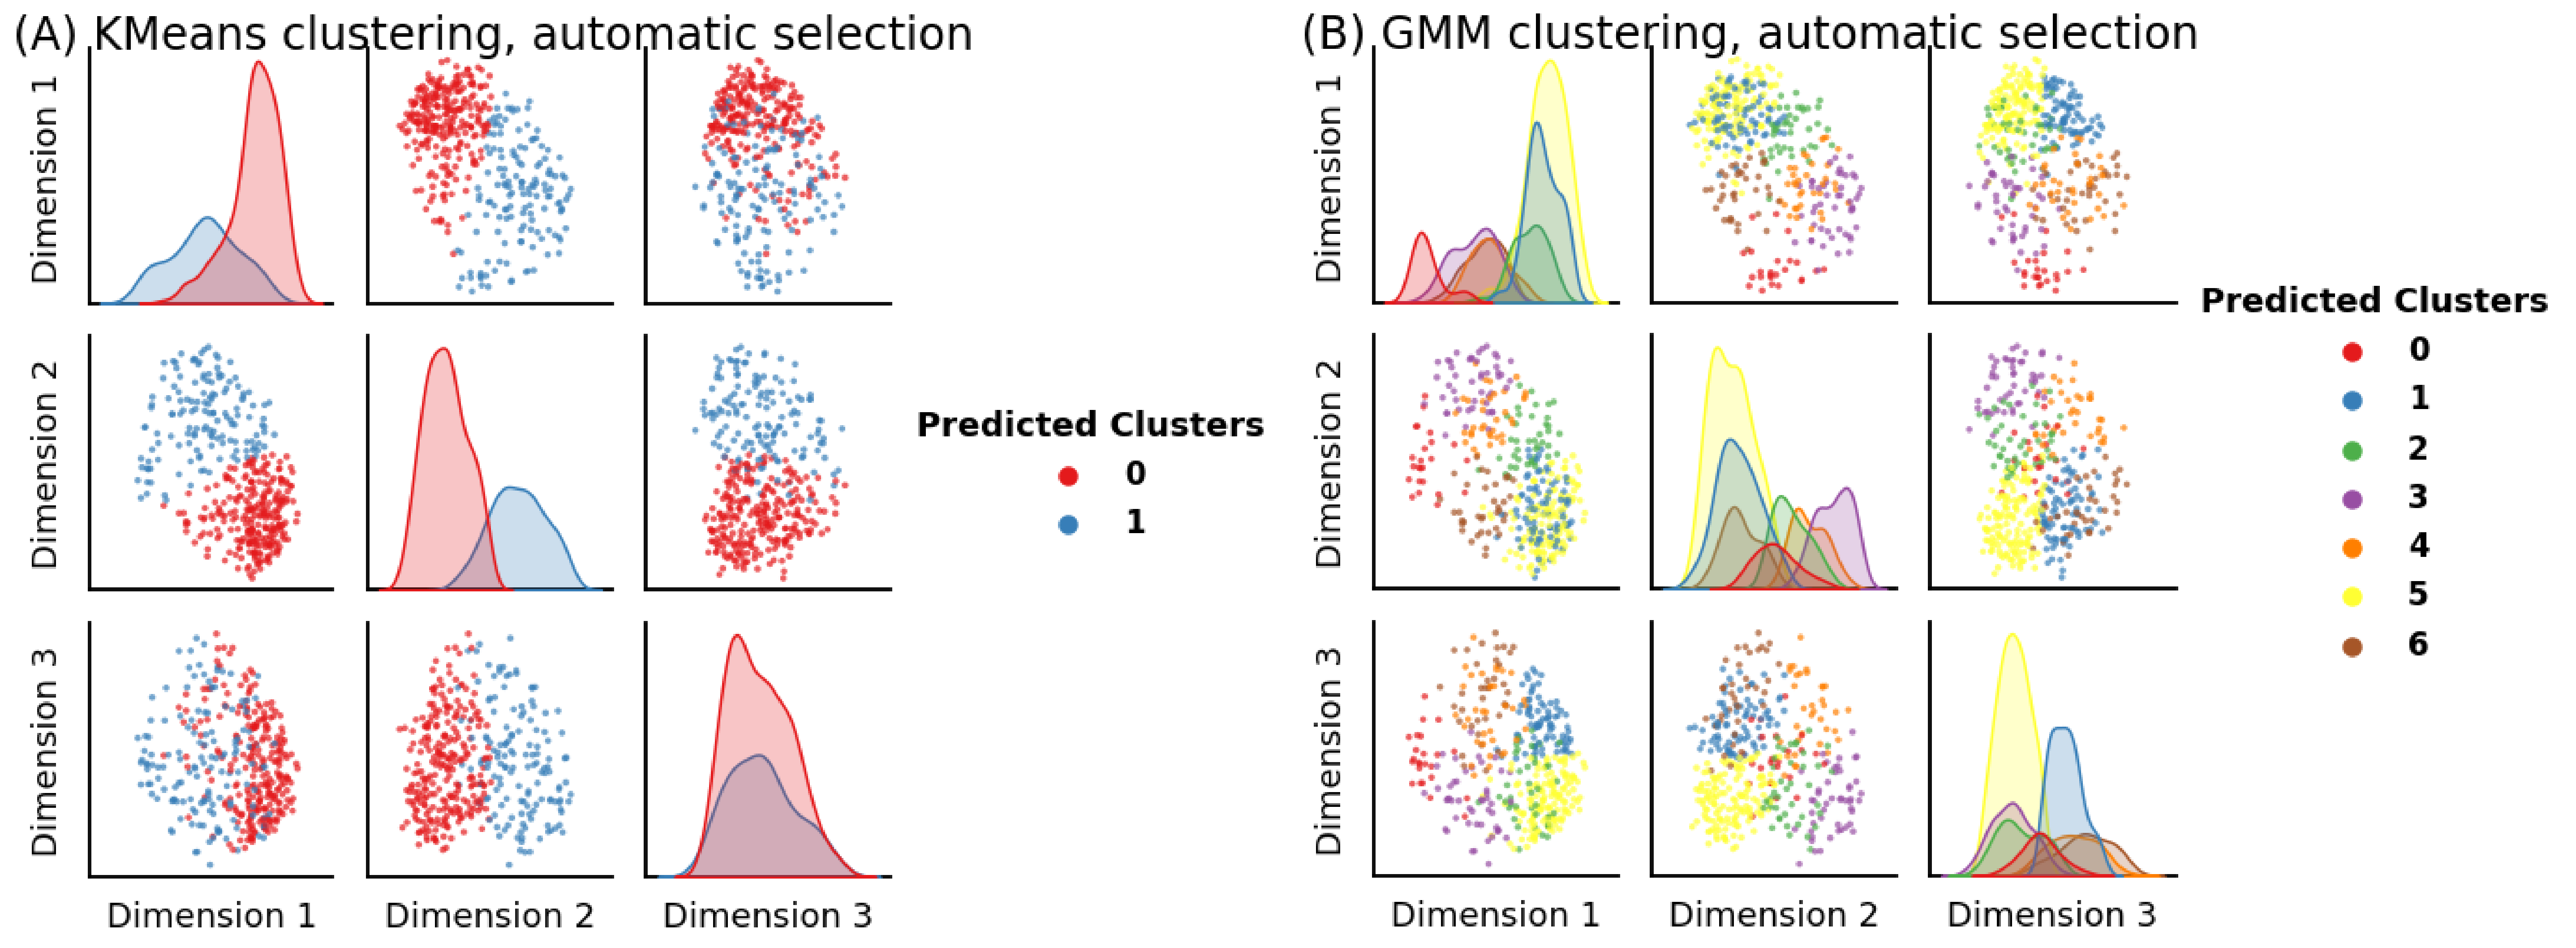
\includegraphics[width=\linewidth]{foundations/ch2/Images/pairplots_impute.png}
    \caption[Comparison of labels estimated by $k$-means and GMM]{\textbf{(A)} the pairs plot for the embedded data, with node communities estimated by \texttt{KMeans}. \textbf{(B)} the pairs plot for the embedded data, with node communities estimated by \texttt{GMM}.}
    \label{fig:ch2:pairplots_impute}
\end{figure}

\newpage
\section{Fine tuning a network machine learning model}
\label{sec:ch2:finetune}

Now that we have figured out an appropriate way to represent our network, and we've gained a few insights, it's time to tune things up a little bit.

In \ref{sec:ch2:select} we saw how to take one of the networks and use embeddings combined with various clustering techniques to learn about latent structure in the data.

However, there's a big caveat: your colleague sent you over a hundred networks, and you ignored all but one of them! Surely, there's something that you can learn from all of them, right?

Fortunately, when you have a multiple network problem, there are plenty of approaches that you can use to learn from all of them simultaneously. Let's break down how we can approach this.

You want to produce a representation of all of your networks. These networks all have the same nodes, which are the different areas of the brain. For all intents and purposes, you can assume that these different nodes mean the same thing across all of the different people, even if they are different based on each individual. What you want to learn is whether there is some {shared} structure across all of the different networks present in the nodes. To do this, you are going to want to be able to take {all} of your networks, and produce an embedding in which you can look at each {node} as its own object. Does anything exist to help you?

There sure does. A particular representation called \texttt{MASE} from Section \ref{ch6:multinet:mase} does just this. It allows you to take many networks, and learn a single representation for the nodes across all of the networks. This representation, in particular, is going to effectively {borrow strength} from all of the networks you pass in, so you won't have to worry about whether you are just ignoring all of the networks but one like you did before. Let's see what \texttt{MASE} can do for us here:


\begin{lstlisting}[style=python]
from graspologic.embed import MultipleASE

embedding = MultipleASE().fit_transform(As)
_ = pairplot(embedding, title="Multiple spectral embedding of all connectomes")
\end{lstlisting}

Let's take a look at what happens when we apply our clustering to this embedding:

\begin{lstlisting}[style=python]
labels = AutoGMMCluster(max_components=10).fit_predict(embedding)
_ = pairplot(embedding, labels=labels,
                title="Multiple spectral embedding of all connectomes", 
                legend_name="Predicted Clusters")
\end{lstlisting}
The pairs plot of the \texttt{MASE} embedding with labels estimated by \texttt{GMM} is shown in Figure \ref{fig:ch2:mase}. Again, the clustering algorithm applied has some element of randomness to it, so don't be concerned if you don't get the exact same number of predicted clusters as we did, or if your clusters look a little different.

\begin{figure}[h]
    \centering
    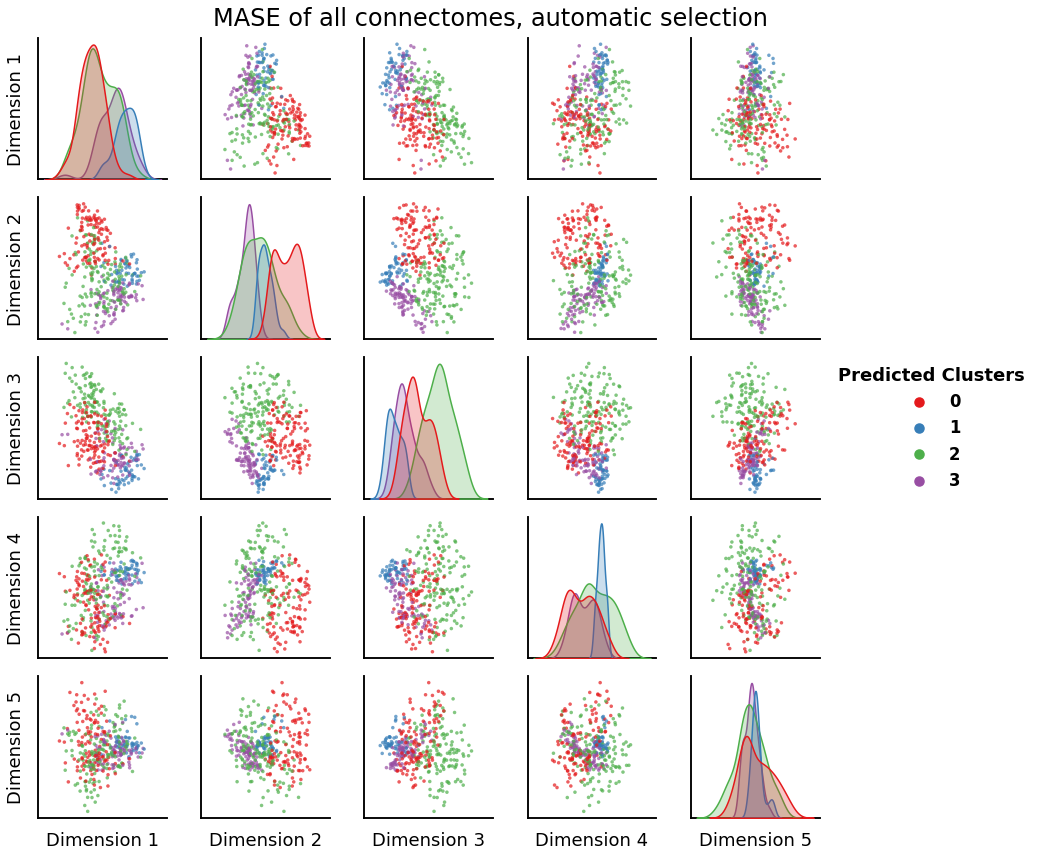
\includegraphics[width=\linewidth]{foundations/ch2/Images/mase.png}
    \caption[Joint embedding with estimated labels for connectomes]{\textbf{(A)} The \texttt{MASE} embedding, which learns an embedding across all networks in your dataset. \textbf{(B)} The \texttt{MASE} embedding, with labels learned by \texttt{GMM}.}
    \label{fig:ch2:mase}
\end{figure}
\newpage
\section{Discover and visualize the system to gain insights}
\label{sec:ch2:discover}

So, now we've got a codebase accumulated to read in the input data, get it cleaned up, embed it while borrowing strength from all networks, and make some predictions. 

So, now we're finished, right?

Wrong! The end of a computational analysis typically means the fun is just beginning: it's now time to \emph{make sense} of whatever, exactly, it is that you just did!

How could we visualize the node clusters (or, more formally, called \emph{communities}) that we just made? We already known about the pairs plot, which we saw in Figure \ref{fig:ch2:mase}(B). 

What if we take a look at the nodes, which if we remember were areas of the brain, and visualize how they \emph{really} look in the brain's natural space?

It turns out that the areas of the brain corresponding to the nodes in your network are, in fact, \emph{known} 3D points in the brain. This means that, with some minor work, we can figure out the coordinates of the individual nodes for the brain. Let's use the neuroparc repository from \cite{Lawrence2021Mar} to grab the 3D coordinates of each node in the network. You don't need to worry too much about how this code works; at a high-level, it just obtains 3D coordinates for the nodes of the network in a \texttt{json} file, and then parses them into a \texttt{pandas} dataframe:


\begin{lstlisting}[style=python]
from urllib import request
import json
import pandas as pd

coord_dest = os.path.join(FMRI_PATH, "coordinates.json")
request.urlretrieve("https://github.com/neurodata/neuroparc/" + "raw/master/atlases/label/Human/Metadata-json/" + parcellation + "_space-MNI152NLin6_res-2x2x2.json", coord_dest);

with open(coord_dest) as coord_f:
    coords = []
    for roiname, contents in json.load(coord_f)["rois"].items():
        try:
            if roiname != "0":
                coord_roi = {"x" : contents["center"][0], "y" : contents["center"][1], "z" : contents["center"][2]}
                coords.append(coord_roi)
        except:
            continue
            
coords_df = pd.DataFrame(coords)
\end{lstlisting}

Now that we have the coordinates, let's try plotting the nodes, but in their native spatial orientation. Here, the color will indicate the predicted label, from our clustering. The slices we'll show will be a saggital slice through the brain. A saggital slice shows the brain nodes oriented from back (right of the plot) of the brain to front (left of the plot), and from bottom (bottom of the plot) to top (top of the plot). On the left, we show the brain with the lobe annotations, and on the right, the predicted labels of each node in color, where each node is shown in its true physical location:

\begin{lstlisting}[style=python]
import matplotlib.image as mpimg

coords_df["Community"] = labels
coords_df['Community'] = coords_df['Community'].astype('category')
fig, axs = plt.subplots(1, 2, figsize=(18, 6))
axs[0].imshow(mpimg.imread('./Images/lobes.png'))
axs[0].set_axis_off()
sns.scatterplot(x="y", y="z", data=coords_df, hue="Community", ax=axs[1])
\end{lstlisting}
\begin{figure}[h]
    \centering
    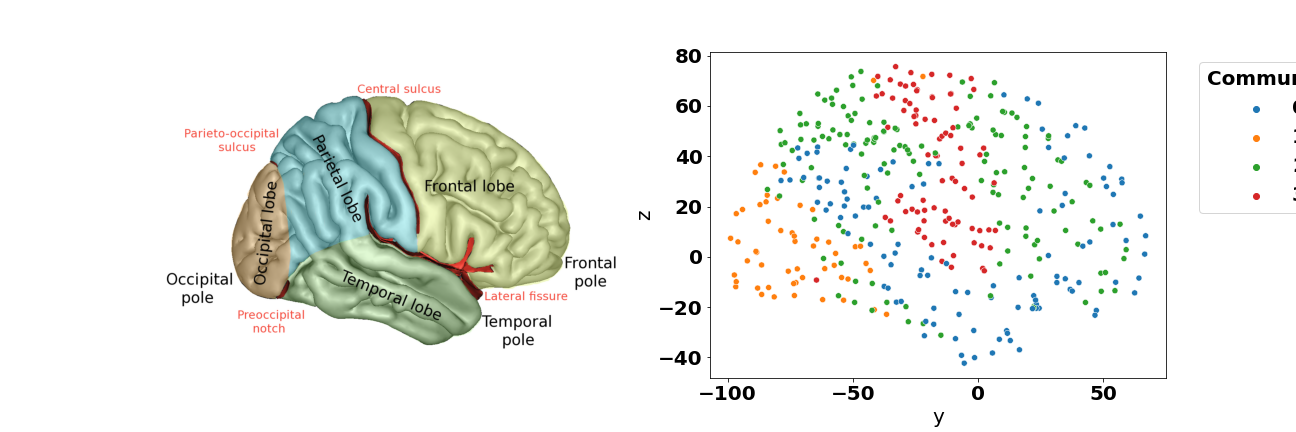
\includegraphics[width=\linewidth]{foundations/ch2/Images/brain_preds.png}
    \caption[Visualizing estimated node communities in 3D space]{Visualizing the estimated node communities with brain lobe annotations.}
    \label{fig:ch2:brain_preds}
\end{figure}

The resulting plot is shown in Figure \ref{fig:ch2:brain_preds}. So, the estimated communities of each node don't quite perfectly align with the brain lobe that the node is in. However, nodes in the tend to be \emph{spatially close} to other nodes in the same estimated community. Notice, for instance, that a lot of nodes in the left side of the brain, the part marked ``occipital lobe'' in the plot, tend to be the same color. In our plot, these nodes are orange; in your plot, they might be a different color. 

In neuroimaging, there tend to be ``groups'' of brain areas that work together, which are organized in files called ``parcellations''. The idea is that they ``parcellate'' (segment) different areas of the brain baesd on two factors: whether the areas of the brain work together, and whether they are located near each other in the brain. Let's see how well the labels we obtained align with these parcellations. We'll do this by looking at the different parcellations (there are $7$ of them in the one that we will use here), and count the number of nodes in a given community (the thing that you just estimated, indicated by color, above) that are assigned to a particular parcel as well. This means that we will end up with a matrix where the number of rows are the number of true parcels in the brain, the number of columns is the number of predicted communities that you found above, and the entries of the matrix are the counts of nodes in the network that are assigned to a given community \emph{and} fall into a given parcel:

\begin{lstlisting}[style=python]
import contextlib
import datasets.dice as dice
from sklearn.metrics import confusion_matrix
from graphbook_code import cmaps

group_dest = os.path.join("./datasets/", "Yeo-7_space-MNI152NLin6_res-2x2x2.nii.gz")
request.urlretrieve("https://github.com/neurodata/neuroparc/" + "blob/master/atlases/label/Human/" +
"Yeo-7_space-MNI152NLin6_res-2x2x2.nii.gz?raw=true", group_dest);
roi_dest = os.path.join("./datasets/", "Schaefer200_space-MNI152NLin6_res-2x2x2.nii.gz")
request.urlretrieve("https://github.com/neurodata/neuroparc/" + "blob/master/atlases/label/Human/" + "Schaefer400_space-MNI152NLin6_res-2x2x2.nii.gz?raw=true", roi_dest);

dicemap, _, _ = dice.dice_roi("./datasets/", "./datasets", "Yeo-7_space-MNI152NLin6_res-2x2x2.nii.gz", 
              "Schaefer200_space-MNI152NLin6_res-2x2x2.nii.gz", verbose=False, plot=False)
actual_cluster = np.argmax(dicemap, axis=0)[1:] - 1

# make confusion matrix
cf_matrix = confusion_matrix(actual_cluster, labels)

# and plot it
ax = sns.heatmap(cf_matrix, cmap=cmaps["sequential"])
ax.set_title("Confusion matrix")
ax.set_ylabel("True Label")
ax.set_xlabel("Predicted Label")
\end{lstlisting}

\begin{figure}[h]
    \centering
    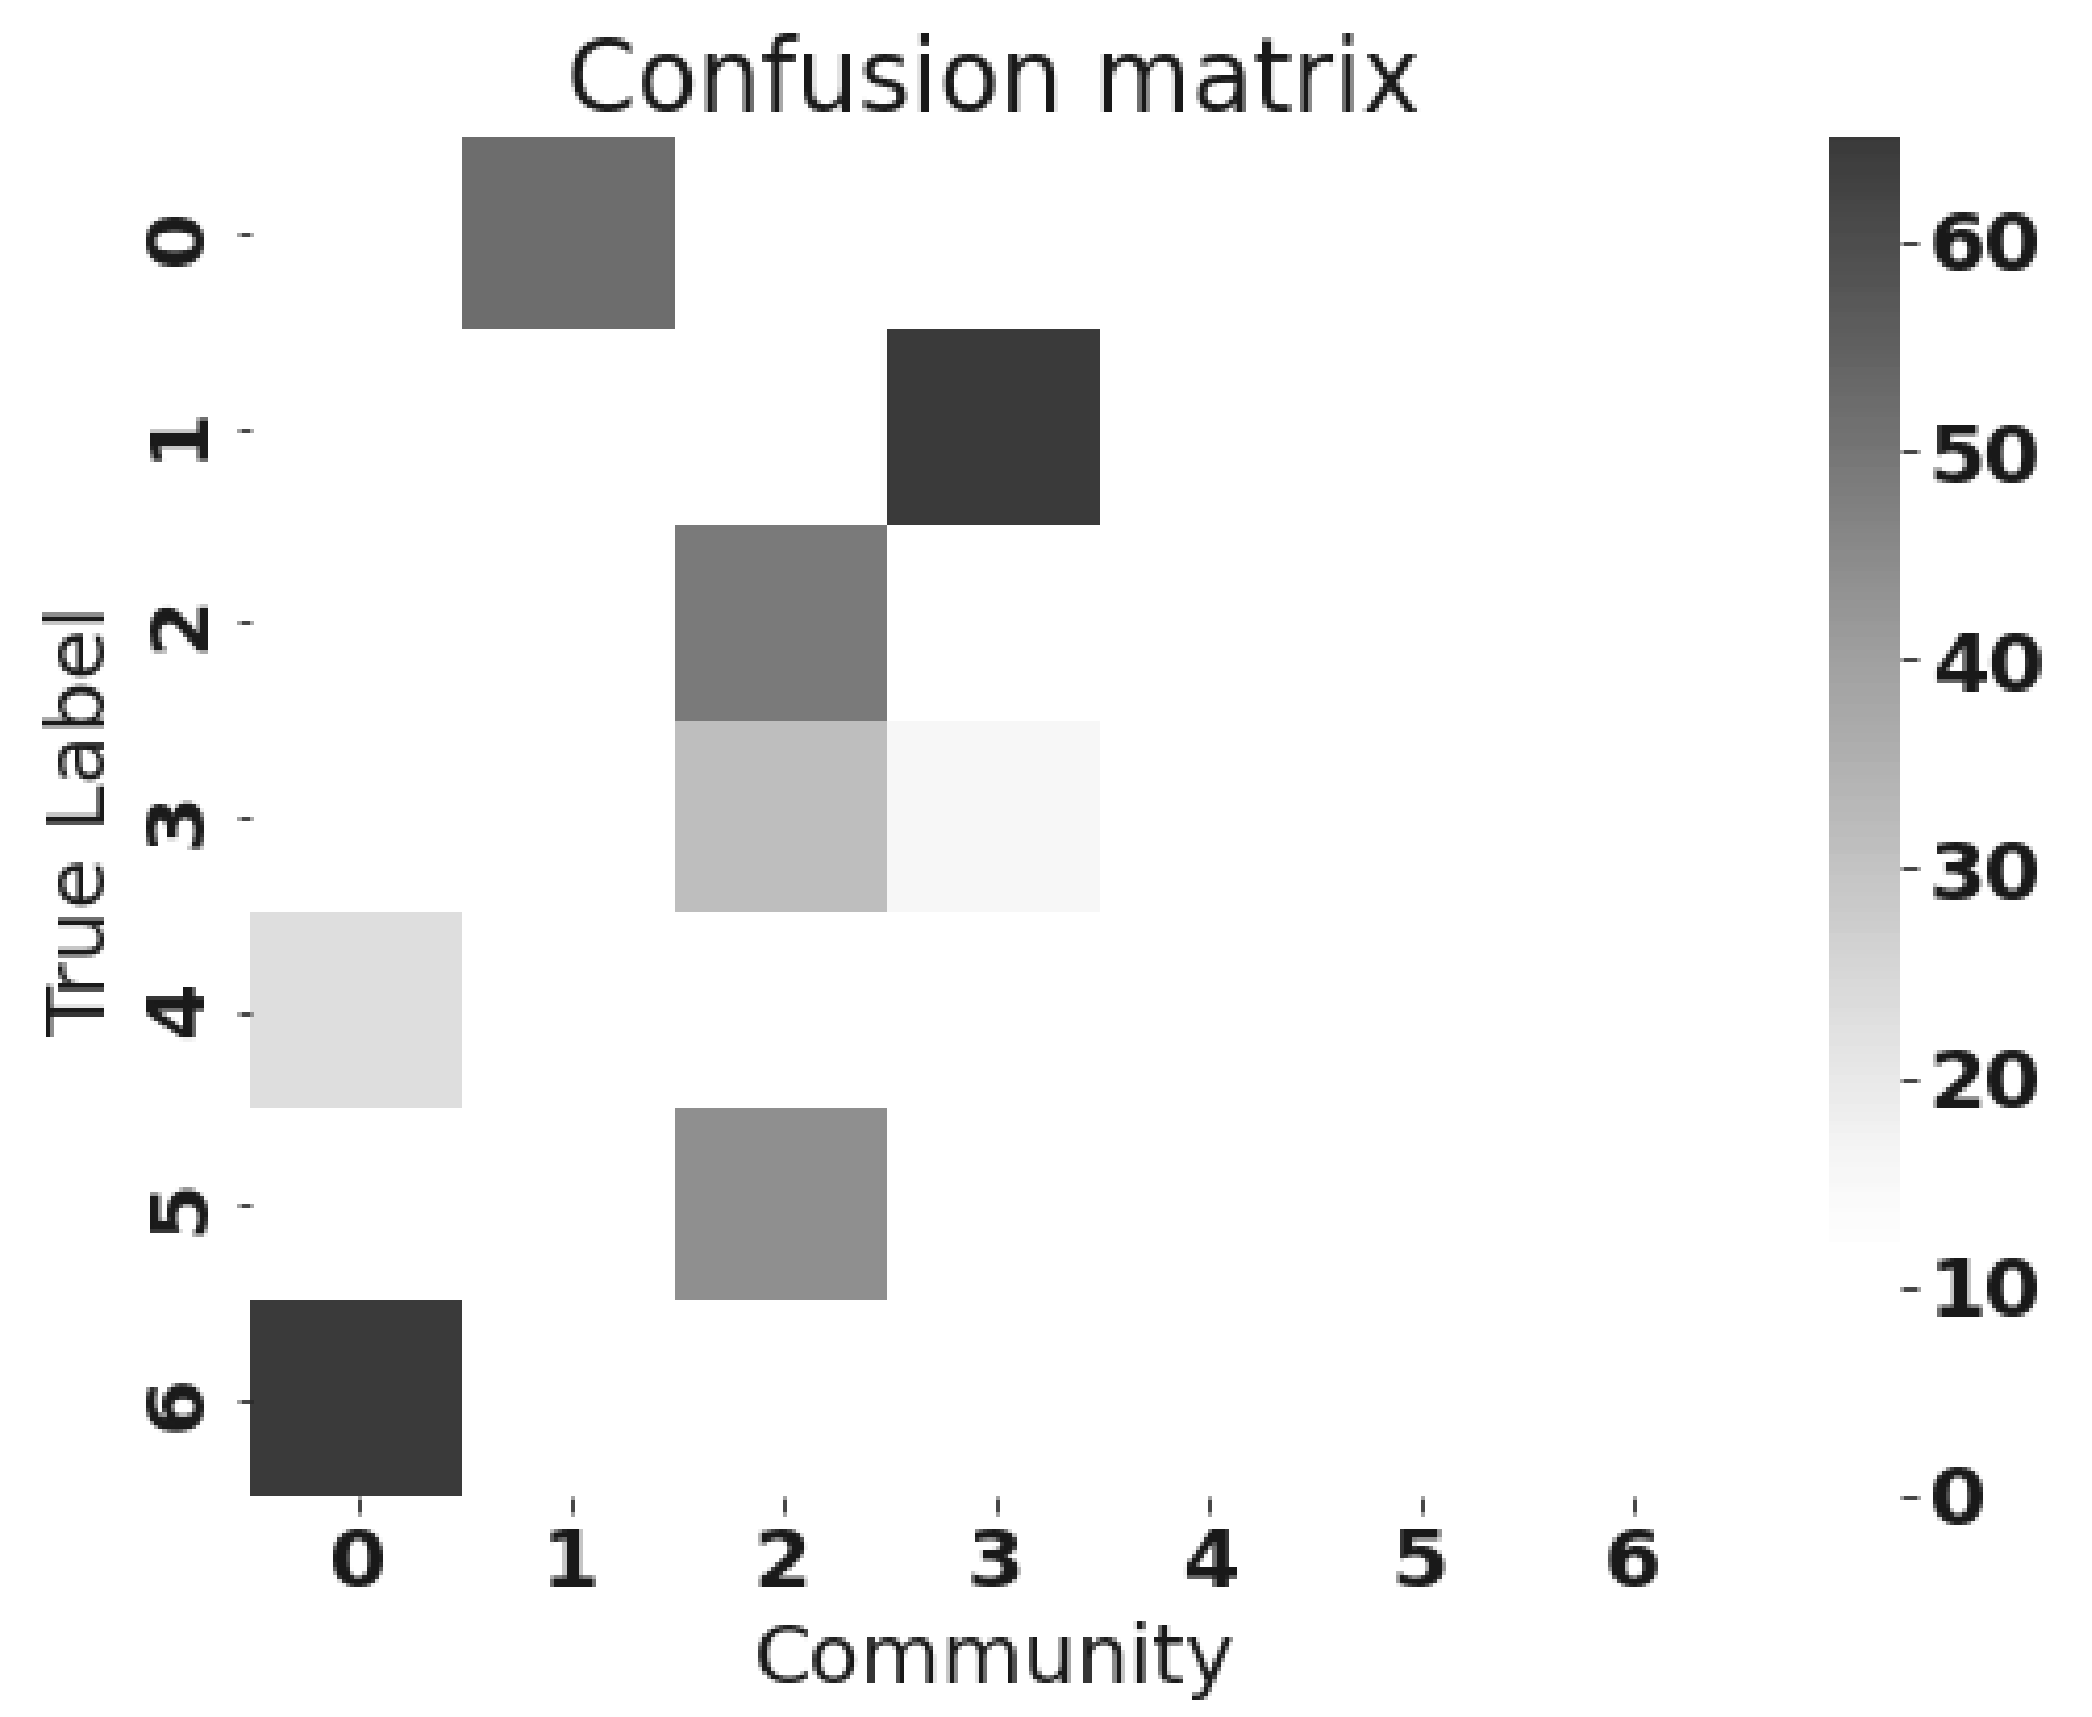
\includegraphics[width=0.5\linewidth]{foundations/ch2/Images/cf_mtx.png}
    \caption[Confusion matrix for node predictions]{The confusion matrix of the estimated clusters for each node in the networks, compared to the lobe that each node is in.}
    \label{fig:ch2:cf_mtx}
\end{figure}
The resulting plot is shown in Figure \ref{fig:ch2:cf_mtx}. in As you will learn in the section on \texttt{MASE} embedding in Section \ref{ch6:multinet:mase}, the mase embedding followed by clustering tends to find groups of nodes that have similar connectivity patterns in the connectomes (it will do a good job at finding the nodes that work together). This means that the nodes in the same community tend to behave ``as a unit'', if you will, in that they tend to be active/inactive together. Basically, what the plot above shows is that nodes that tend to have similar connectivity patterns (from the networks) tend to also be in the same parcel (the \emph{true label}), which makes sense since the parcels are based on connectivity profiles from brains. The clustering isn't \emph{perfect}, in that it is never the case that a single predicted label corresponds to \emph{exactly} one true label. If that were the case, we would expect for each column in the above ``confusion matrix'' to only have one possible true label that nodes within this predicted label are assigned to, which isn't quite the case. 

Taking these conclusions together, we find that some areas of the brain (such as the occipital and parietal areas) feature nodes which are both functionally \emph{and} spatially similar: they tend to show similar connectivity patterns with respect to other groups of nodes in the network, \emph{and} are in similar spatial positions in the brain. On the other hand, for other areas of the brain, while the nodes may be functionally similar, they might not necessarily be spatially similar. This is where the domain expertise kicks in: we don't know how to interpret this particular aspect of our finding, but maybe you or your colleagues do!

Further, while this analysis \emph{only} really ended up looking at whether different groups of nodes worked together, there's really no reason we couldn't \emph{also} incorporate spatial information about the nodes into our analysis. In Section \ref{ch6:joint}, you will learn some techniques for incorporating both the network data itself and other information about the nodes into your analysis through a technique called Covariate-Assisted Spectral Embedding (\texttt{CASE}), such as spatial information.

And this is where the fun of network machine learning comes into play: it is a tool not only to \emph{apply} algorithms to data, but to facilitate \emph{learning new things} about that data as well. You might get some predictable conclusions (such as some of the nodes being both functionally and spatially similar), and you might get some unpredictable conclusions (such as some of the nodes being functionally, but \emph{not} spatially, similar). Your ability to understand network machine learning, while crucial, is going to go \emph{hand in hand} with your ability to understand the intricacies of the domain you want to apply network machine learning to. We hope that we can help with the former part; we'll leave the latter to you!

\subsection{Try it out}

Hopefully this chapter gave you a small scale peek at what a network machine learning project looks like, and showed you a brief introduction to some tools you can use to gain novel insights from your network data. While what we did in this chapter was relatively straightforward, the process from obtaining your data to choosing appropriate network machine learning problems can be extremely arduous! In fact, as a network machine learning scientist, you might find that just obtaining your data in a useful form (a network) and cleaning the data to be usable might take an \emph{enormous} chunk of your time!

If you haven't already done so, now is a fantastic time to grab your laptop, select a network dataset you are interested in, and start trying to work through the whole process from A to Z. If you need some pointers, the \texttt{graspologic} package makes several datasets available to you \cite{graspydata}. We'd recommend working through the contents of this book by first using the example data that is presented in the chapter, and then try to apply the techniques to a network dataset of your choosing.

\bibliographystyle{vancouver}
\bibliography{references}